\documentclass[11pt]{article}

\usepackage{algpseudocode,lineno}
\usepackage{enumitem}
\usepackage{amssymb,multirow,color,comment,amsmath}
\usepackage{amsfonts,amsthm, bm}
\usepackage{xcolor}
\usepackage[font=itshape]{quoting}
\usepackage{algorithm,algpseudocode}
\usepackage{verbatim}
\usepackage{amssymb,multirow,color,comment,amsmath}
%% The amsthm package provides extended theorem environments
\usepackage{amsthm,tikz}
\usetikzlibrary{matrix}
\usepackage{pgfplots,cite}
\usepackage{subfigure,bm}
\usepackage{algorithm,algpseudocode}
\usepackage{breqn}
\usepackage[font=itshape]{quoting}

\usepackage[margin=1.4in]{geometry}

\usetikzlibrary{arrows,calc}
\usepackage{multirow,comment}
\usepackage{pgf,tikz,tikz-3dplot}
\usepackage[percent]{overpic}
\usepackage{pdflscape}
\usepackage{pgfplots,xcolor} 
\usepackage[makeroom]{cancel}
\numberwithin{equation}{section}
% %% The amsthm package provides extended theorem environments
% \usepackage{amsthm,tikz}
% \usetikzlibrary{matrix}
% \usepackage{pgfplots}
% \usepackage{subfigure,bm}
% \usepackage{breqn}

% \usetikzlibrary{arrows,calc}
% \usepackage{multirow,comment,enumerate}
% \usepackage{pgf,tikz,tikz-3dplot}
% \usepackage[percent]{overpic}
% \usepackage{pdflscape}
% \usepackage{pgfplots,xcolor, minted} 
% \usepackage[makeroom]{cancel}
\newcommand{\bE}{\mathbf{E}}
\newcommand{\br}{\mathbf{r}}
\newcommand{\sd}{\mbox{d}}
\newcommand{\te}{\mbox{e}}
\newcommand{\bP}{\mathbf{P}}
\newcommand{\bJ}{\mathbf{J}}
\newcommand{\bd}{\mathbf{d}}
\newcommand{\bx}{\mathbf{x}}
\newcommand{\bn}{\mathbf{n}}
\newcommand{\by}{\mathbf{y}}
\newcommand{\red}[1]{{\color{black} #1}}
\DeclareMathAlphabet\mathbfcal{OMS}{cmsy}{b}{n}

\begin{document}

% \title[JASA/Sample JASA Article]{Accelerating numerical methods for \\
% nonlinear acoustics using nested meshes}
\title{\red{Accelerating frequency-domain numerical methods for 
weakly nonlinear focused ultrasound using nested meshes}}
\author{Samuel P.~Groth$^1$, Pierre G\'{e}lat$^2$, Seyyed R.~Haqshenas$^{2}$, \\ 
Nader Saffari$^2$, Elwin van 't Wout$^3$, Timo Betcke$^4$, Garth N.~Wells$^1$\\[6pt]
$^1$Department of Engineering, University of Cambridge \\[4pt] %, Cambridge CB2 1PZ, United Kingdom 
$^2$Department of Mechanical Engineering, University College London, \\[4pt] %\\ London WC1E 7JE, United Kingdom 
$^3$Institute for Mathematical and Computational Engineering, \\
School of Engineering and Faculty of Mathematics, \\
            Pontificia Universidad Cat\'olica de Chile \\ [4pt]
$^4$Department of Mathematics, University College London} %, Santiago, Chile}
% \email{samuelpgroth@gmail.com}
% \affiliation{Department of Engineering, University of Cambridge, Cambridge CB2 1PZ, United Kingdom}
% \author{Pierre G\'{e}lat}
% \author{Seyyed R.~Haqshenas}
% \author{Nader Saffari}
% \affiliation{Department of Mechanical Engineering, University College London, London WC1E 7JE, United Kingdom}
% \author{Elwin van 't Wout}
% \affiliation{Institute for Mathematical and Computational Engineering,
% School of Engineering and Faculty of Mathematics,
%             Pontificia Universidad Cat\'olica de Chile, Santiago, Chile}
% \author{Timo Betcke}
% \affiliation{Department of Mathematics, Unversity College London, London WC1H 0AY, United Kingdom}
% \author{Garth N.~Wells$^1$}

% % \preprint{Author, JASA}		%  if you want want this message to appear in upper right corner of title page for preprint only

% \date{\today} 
\maketitle
\begin{abstract}
%     The numerical simulation of nonlinear ultrasound is important in the treatment planning for high-intensity focused ultrasound (HIFU) therapies in the abdomen. However, the large domain sizes and generation of higher harmonics at the focus make these problems computationally demanding. Numerical methods typically employ uniform meshes fine enough to resolve the highest harmonic present in the problem, leading to very large numbers of unknowns. This paper proposes a more efficient strategy in which each harmonic is approximated on a separate mesh, the size of which is proportional to wavelength of the harmonic. The increase in resolution required to resolve a smaller wavelength is balanced by a reduction in the domain size, which is feasible owing to the localised nature of harmonics near the focus. 

% Numerical experiments are performed for HIFU transducers in order to determine the size of the meshes required to represent the harmonics. A volume potential approach is proposed to perform convergence experiments as the computation domain size is reduced. This approach allows each harmonic to be computed rapidly via the evaluation of an integral over the domain. It is shown that at least an order of magnitude reduction in memory consumption and computation time can be achieved.


    The numerical simulation of \red{weakly} nonlinear ultrasound is important in 
    treatment planning for \red{focused ultrasound (FUS)} therapies.
    However, the large domain sizes and generation of higher harmonics at the focus 
    make these problems extremely computationally demanding. Numerical
    methods typically employ a uniform mesh fine enough to resolve the highest harmonic 
    present in the problem, leading to a very large number of degrees of freedom. 
    This paper proposes a more efficient strategy 
    in which each harmonic is approximated on a separate mesh, the size of which
    is proportional to \red{the} wavelength of the harmonic. The increase in 
    resolution required to resolve a smaller wavelength is balanced by a 
    reduction in the domain size. This nested meshing is feasible 
    owing to the increasingly localised nature of higher harmonics near the focus.

    Numerical experiments are performed for \red{FUS} transducers in 
    homogeneous media in order to determine the size of the meshes 
    required to accurately represent the harmonics. In particular, a fast 
    \textit{volume potential} approach is proposed and employed to perform convergence
    experiments as the computation domain size is modified. This approach allows each harmonic to 
    be computed via the evaluation of an integral over the domain. Discretising this 
    integral using the midpoint rule allows the computations to be performed 
    rapidly with the FFT. It is shown that at least an order of magnitude 
    reduction in memory consumption and computation time can be achieved with
    nested meshing. \red{Finally, it is demonstrated how to generalise this approach 
    to inhomogeneous propagation domains.}

\end{abstract}

%% pacs numbers not used


\clearpage
\section{\label{sec:1} Introduction}
\red{Focused ultrasound (FUS)} is a non-invasive tumor ablation 
therapy in which acoustic waves are focused at a target location, thereby 
elevating the temperature sufficiently to destroy the tumor tissue. Tissue 
death can be caused directly via thermal ablation, or via other 
mechanisms such as cavitation~\cite{vlaisavljevich2013image,izadifar2017mechanical},
\red{shock-scattering histotripsy~\cite{maxwell2011cavitation}, and boiling histotripsy~\cite{khokhlova2011controlled}}. 
In the thermal ablation setting, which is the focus of this article, the peak acoustic 
pressure is often between 1 and 10 MPa, at which linear acoustic theory is no longer accurate. 
Indeed it has been observed that the contributions from nonlinear effects can
increase the temperature at the focal point by an additional 20\%,
thus substantially reducing the time required for ablation when compared to simulations
using linear theory~\cite{solovchuk2014temperature}.
% Furthermore, the location of the focus in the nonlinear regime is often shifted
% relative to that predicted by the linear theory~\cite{camarena2013nonlinear}. 
To simulate the nonlinear 
acoustic field, a popular model is the Westervelt equation,
which incoporates a quadratic pressure term. Numerically solving the 
Westervelt equation in a \red{FUS} setting is computationally challenging since the
domains are large compared to the smallest wavelength present. 

To put into context the scale of the computational problems presented by 
\red{FUS}, consider a bowl-shaped \red{FUS} transducer with radius 7.5cm and 
geometric focal length 15cm operating at 1.1MHz. 
Transducers of this size are suitable for deep-seated tumors, located in the liver,
for example. A simulation domain spanning the face of the bowl and extending to the 
focal region is approximately 100 wavelengths across in each dimension. If there 
are five harmonics present in the nonlinear field, then this is five hundred 
wavelengths at the fifth harmonic. In order to obtain a reasonable accuracy level,
we can assume that at least six degrees of freedom (DOF) per wavelength are required~\cite{marburg2008discretization}.
Then to simulate this problem in three dimensions, we would require 27 billion 
degrees of freedom. Handling such a large system
presents an enormous computational load in terms of memory and time. 

There has been a great deal of research effort aimed at reducing the computational
cost of nonlinear \red{FUS} simulations. Much of this work employs at least one simplifying assumption, 
such as axisymmetry, one-way wave propagation, or the parabolic approximation
(see \cite{gu2015modeling} for a review). Popular methods for solving 
the original Westervelt equation (or equivalent) include the finite-difference 
time-domain method~\cite{solovchuk2013simulation} (FDTD) and the $k$-space 
pseudospectral method~\cite{treeby2012modeling} (KSPS). Although powerful 
techniques, these full-wave solvers can still yield simulation times in excess 
of a day for realistic problems when run on a large cluster~\cite{jaros2016full}.
% \red{For efficiently simulating highly-focused problems with strong nonlinearities,
% shock-capturing numerical schemes have been developed, however only for 
% the parabolic approximation of the Westervelt equation, known as the KZK equation~\cite{bessonova2009focusing,yuldashev2018wide}.}
\red{For efficiently simulating highly-focused problems with strong nonlinearities,
shock-capturing numerical schemes have been developed and applied for 
the parabolic approximation of the Westervelt equation, known as the KZK equation~\cite{bessonova2009focusing},
wide-angle parabolic approximation~\cite{yuldashev2018wide}, as well as for the 
one-way propagation version of the Westervelt equation~\cite{yuldashev2011simulation}.}

In this paper, we set out to improve upon the meshing strategies employed in 
popular full-wave solvers for the Westervelt equation. \red{These solvers typically use} uniform 
meshes resolved according 
to the wavelength of the highest harmonic. Such a meshing approach is 
inefficient since the higher harmonics are localised around the focus, 
therefore the extremely fine mesh far away from the focus 
is likely overkill. It seems intuitive that a mesh that is gradually refined 
as the focus is approached would be sensible, but at what rate? And what saving 
can one expect to achieve? Here we address these questions via numerical 
experimentation on realistic \red{FUS} transducers taken from \cite{sonic}.

\red{We note similar strategies have previously been employed to reduce the 
computational load of nonlinear acoustics simulations~\cite{yuldashev2011simulation,karzova2017shock}.
In these prior works, it was also observed that far from the transducer focus, higher harmonics provide 
negligible contributions to the acoustic field and therefore, to save on storage requirements, 
higher harmonics are stored only on smaller domains, centred at the focus. However, the grid
step used in these works is not altered for the different harmonic computations. 
By increasing the grid step for lower harmonics, further computational savings can be 
achieved, as we demonstrate in this article. Furthermore, we detail an in-depth 
study of how to choose appropriate computational domains for each harmonic and 
 we provide a useful rule of thumb relating the domain dimensions to each harmonic's wavelength.}


In order to perform these experiments efficiently, we consider a simplified setting 
in which the propagation medium is homogeneous and the signal is assumed to have 
harmonic time dependence. \red{Furthermore, we consider settings in which the peak amplitude 
is no more than 15MPa and thus the field is only weakly non-linear}. Under the time-harmonic 
\red{and weakly non-linear assumptions}, the full-wave Westervelt 
equation reduces to a series of inhomogeneous 
Helmholtz equations, one for each harmonic present in the field (as in, e.g., 
\cite{du2013fast}). %,soneson2017extending}). 
\red{We note that the weak non-linearity permits us to reasonably neglect the 
transfer of energy from higher to lower harmonics. This is, however, not valid for 
extremely high amplitude fields, as encountered in histotripsy applications.}

Since we consider a homogeneous medium, each Helmholtz equation is exactly solved 
by the evaluation of the appropriate \textit{volume potential} integral~\cite{costabel2015spectrum}. 
Therefore, 
for each harmonic in the field, we look at the convergence of the volume potential 
as the domain of integration is increased. In order to efficiently evaluate the 
volume potential, we discretise the domain over a uniform voxel mesh, which allows the 
summation (i.e., the discrete form of the integration) to be performed rapidly 
using the fast-Fourier transform (FFT). This is an extremely efficient technique 
for computing high-order harmonics in a homogeneous medium and its application in 
this area is, to the best of the authors' knowledge, novel.

For numerical investigations with different transducer configurations and within 
two different media (water and liver), we deduce that (for the configurations 
considered) in order to perform accurate computations of the second harmonic, the computation 
domain must extend all the way back to the transducer, however may be contracted 
slightly in the transverse direction. For the third and higher harmonics, the 
computation domain may be contracted in both the axial and transverse directions, 
thus leading to substantial computational savings. In fact, we demonstrate that 
an accurate approximation (less than 1\% relative error) may be obtained while 
contracting the width and length
of the domain in proportion to the wavelength of the harmonic. Thus the number
of cells in every mesh is roughly equal. This amounts to a reduction in 
the number of DOF by a factor of approximately $(n/2)^3$, where $n$ is the number of harmonics 
being computed.

In practice, this leads to a series of nested meshes, each at the resolution
required for the appropriate harmonic and all with the same number of voxels.
To perform computations for higher harmonics, solutions from lower harmonics are 
interpolated onto the finer meshes. We outline an algorithm for this more 
efficient computation of all the harmonics in Section~\ref{subsec:interpolation}
and examine its performance.

The layout of the paper is as follows. Section~\ref{sec:nonlinear_acoustics}
outlines the mathematical model we employ for our \red{FUS} setup. In particular we 
consider the Westervelt equation and review how it reduces to a series of Helmholtz 
equations under the time-harmonic assumption. We further simplify the equations
via an assumption of weak nonlinearity. In Section~\ref{sec:volume} we 
describe how, in the homogeneous domain case, the Helmholtz equations are solved 
exactly via volume potentials. It is then described how these volume potentials 
are efficiently approximated using a voxelised discretisation 
approach. This leads to the discrete versions of the volume potentials having 
block-Toeplitz form; thus the potentials may each be evaluated using 
a single fast matrix-vector product with the FFT. Section~\ref{subsec:incident} 
discusses our model for the time-harmonic bowl-shaped transducer.
Section~\ref{sec:validation} 
presents a validation of our approach by comparing to simulations performed 
with the HITU Simulator \textsc{Matlab} toolbox~\cite{HITUwebpage,soneson2017extending}.
In Section~\ref{sec:results} we perform convergence tests for each of the 
harmonics for a range of problem setups. We present our findings on the rates 
of convergence of the approximation as the domain is increased and present a rule 
of thumb for designing the meshes to ensure each harmonic is accurately 
approximated. In Section~\ref{subsec:interpolation} we present how the hierarchy 
of meshes is used in practice with our volume potential approach, including the 
interpolation of approximations between the meshes. Here we present some performance 
details for this three-dimension full-wave approach on a single workstation.
Finally, in Section~\ref{sec:conclusion} we 
present our conclusions and discuss the relevance of this work to other numerical 
techniques for \red{FUS}.



\section{\label{sec:2} Nonlinear acoustics in the frequency domain}
\label{sec:nonlinear_acoustics}
Acoustic fields produced by \red{FUS} transducers are commonly modelled by the 
Westervelt equation~\cite{hamilton1998nonlinear}:
    \begin{equation}
        \nabla^2 p
        - \frac{1}{c_0^2}\frac{\partial^2 p}{\partial t^2} 
        - \frac{2\alpha_0}{c_0^{1-\eta}}\frac{\partial }{\partial t}
        \left( -\nabla^2\right)^{\eta/2}p = 
        -\frac{\beta}{\rho_0 c_0^4}\frac{\partial^2 p^2}{\partial t^2},
        \label{eqn:west_fractional}
    \end{equation}
    where $p$ is the acoustic pressure, $c_0$ is the speed of sound, 
    $\rho_0$ is the medium density, $\beta$ the non-linearity parameter, and 
    $\alpha_0$ and $\eta$ are medium specific attenuation parameters.    
    The fractional Laplacian appearing in (\ref{eqn:west_fractional}) was first 
    introduced in \cite{chen2004fractional} in order to incorporate frequency 
    dependent power law attenuation. More specifically, in the frequency domain, it 
    generates a complex wavenumber of the form
    \begin{equation}
        k = \frac{\omega}{c_0} + \text{i}\alpha;\quad  \alpha=\alpha_0|\omega|^{\eta},
        \label{eqn:power_law}
    \end{equation}
    for $\alpha_0|\omega|^{\eta-1}c_0<0.1$ ~\cite{szabo1994time}, where $\omega$
    is the angular frequency of the transducer.
    The power law exponent is typically in the range 
    $1\leq \eta\leq 2$. We note that this power law attenuation can also be incorporated 
    via a temporal convolution, as was originally proposed in \cite{szabo1994time}; 
    we refer the reader to \cite{treeby2010modeling} for a review of power law 
    attenuation techniques. \red{We note that the relation (\ref{eqn:power_law}) does not 
    incorporate the effect of dispersion on the real part of the wavenumber. However,
    for the frequencies and materials considered in this article, this effect is negligibly
    small. For highly nonlinear and higher frequency problems, the relation may be 
    modified to more accurately incorporate dispersion, as discussed in \cite{treeby2010modeling,waters2005causality}.}
    
In this article, we assume that the operation time of the transducer is long
when compared to the period of the signal. Therefore, the total acoustic 
pressure can be written as the following sum over harmonics 
(as in \cite{du2013fast,soneson2017extending}):
\red{
\begin{equation}
    p(\bx, t) = \text{Re} \left\{\sum_{n=1}^{\infty} 
        p_n(\bx)e^{-\text{i}n\omega t}\right\}.
    \label{eqn:time_harm_real}
\end{equation}
} 
Many numerical schemes in the literature consider the time-harmonic form 
(\ref{eqn:time_harm_real}), e.g., \cite{campos1999finite, du2013fast,soneson2017extending,
van2015fast}, likely owing to the distinct advantages of a frequency domain 
approach:
\begin{itemize}
    \item the challenging task of choosing/developing an efficient time stepping 
    scheme can be avoided; 
    \item arbitrary frequency-dependent attenuation power laws can be easily incorporated
    (whereas in the time domain one has to contend with the fractional Laplacian);
    \item methods such as the boundary element method 
    and volume integral equation method, can be applied directly;
    \item the computation regions for higher harmonics can 
    be reduced, thereby making simulations more efficient.
\end{itemize}
It is this final point that we study in this article.
    
The form (\ref{eqn:time_harm_real}) is not well suited for 
substitution into (\ref{eqn:west_fractional}) 
since the right-hand of (\ref{eqn:west_fractional}) requires the computation of 
a product. For such a product, expressions in which real or imaginary parts are 
required to be taken lead to cumbersome algebra. Therefore, it is more 
straightforward to use the following expression, which is equivalent to 
(\ref{eqn:time_harm_real}):
\begin{equation}
    p(\bx,t) = \frac{1}{2}\sum_{n=1}^{\infty}\left(p_n(\bx)e^{-\text{i}n\omega t} + 
                                       p_n^*(\bx)e^{\text{i}n\omega t}\right),
    \label{eqn:cc}
\end{equation} 
where $^*$ denotes complex conjugation.
Substituting (\ref{eqn:cc}) into (\ref{eqn:west_fractional}) and matching 
coefficients of $e^{-\text{i} n\omega t}$ for $n\geq 1$ yields  
\begin{equation}
    \nabla^2 p_n 
    + k_n^2 p_n = \frac{\beta\omega^2}{2\rho_0 c_0^4}n^2
    \sum_{m=1}^{\infty}p_m(p_{n-m}+2p^*_{m-n}),
    \label{eqn:cascade_1}
\end{equation}
for $n=1,2,\ldots$, where $p_n = 0$ for $n\leq 0$, and the complex wavenumbers are defined as 
\begin{equation}
    k_n = \frac{n\omega}{c_0} + \text{i}\alpha(n\omega).
\end{equation}
    
The equations (\ref{eqn:cascade_1}) can be further simplified by neglecting 
small terms on the right-hand side, which is appropriate in the weakly nonlinear
case, as was considered in, e.g., \cite{du2013fast}. Specifically, we neglect all terms $p_ip_j$
and $p_ip^*_j$ for which $i+j>n$, for $n=1,2,\ldots$, thus giving
\begin{equation}
    \nabla^2 p_n
    + k_n^2 p_n = \frac{\beta\omega^2}{2\rho_0 c_0^4}n^2
    \sum_{m=1}^{n-1}p_m p_{n-m}.
    \label{eqn:cascade_2}
\end{equation}
This is a cascade of inhomogeneous Helmholtz equations in which each right-hand 
side is a combination of products of lower harmonics. Therefore, we can solve 
the equations sequentially, starting from $n=1$.

We note that the assumption of weak nonlinearity is valid for a range of 
\red{FUS} applications for thermal ablation, \red{for example, at a preclinical stage, 
when excitation protocols and devices require characterisation~\cite{kothapalli2018convenient,ries2010real}.} 
However, for extremely high focal pressures such as those encountered in \red{lithotripsy and histotripsy, where pressures much higher 
than 30MPa can be seen~\cite{izadifar2017mechanical}}, the terms neglected above become significant. 
Therefore, a modified approach would be required, however we do not consider 
this case here.

%%%%%%%%%%%%%%%%%%%%%%%%%%%%%%%%%%%%%%%%%%%%%%%%%%%%%%%%%%%%%%%%%%%%%%%%%%%%%%%
\section{Volume potentials}
\label{sec:volume}
The equations (\ref{eqn:cascade_2}) are each of the general form
\begin{equation}
    \nabla^2 u + k^2 u = f(\bx), \quad \bx\in\mathbb{R}^3.
    \label{eqn:helmholtz}
\end{equation}
Via Green's theorem (see, e.g., \cite{colton2013integral,costabel2015spectrum})
it can be seen that the following volume potential satifies (\ref{eqn:helmholtz}):
\begin{equation}
    u(\bx) = -\int_{\mathbb{R}^3}G_k(\bx,\by)f(\by)\sd \by, \quad \bx\in\mathbb{R}^3,
    \label{eqn:vol_pot}
\end{equation}
where $G_k$ is the fundamental solution to the Helmholtz equation, also known as 
Green's function:
% \footnote{We 
% note that the fundamental solution has the property 
% $\nabla^2 G(\bx,\by) + k^2G(\bx,\by) = -\delta(\bx-\by)$.}
\begin{equation}
    G_k(\bx,\by)=\frac{e^{\text{i} k|\bx-\by|}}{4\pi|\bx-\by|},\quad \bx\neq\by.
    \label{eqn:green}
\end{equation}
\red{This function is singular when $\bx=\by$, however integrals of the function
across this singularity may be be evaluated using principal value techniques or 
appropriate coordinate transformations, as we shall see in Section~\ref{ss:compute_potential}.}
We note that the integral in (\ref{eqn:vol_pot}) is over an infinite domain, 
however in practice we replace this with a finite domain of integration, $D$.
So we have that 
\begin{equation}
    u(\bx) = -\int_{D}G_k(\bx,\by)f(\by)\sd \by + \varepsilon(D), \quad \bx\in D\subset\mathbb{R}^3,
    \label{eqn:vol_pot_approx}
\end{equation}
where $\varepsilon(D)$ an error incurred by the introduction of a finite integration
domain. Since the \red{FUS} field is highly focused, a sensibly chosen finite $D$ will 
yield a negligibly small error. It is the purpose of this article to investigate how small $D$ 
can be made whilst still yielding accurate approximations to $u$.

For clarity, we write out this integral representation (\ref{eqn:vol_pot_approx})
for each of the first five harmonics:
\begin{align}
    \label{eqn:harm2} p_2(\bx) &= -\frac{2\beta \omega^2}{\rho_0 c_0^4}
                    \int_{D_2}G_{k_2}(\bx,\by)p_1^2(\by)\sd \by, \\
        \label{eqn:harm3} p_3(\bx) &= -\frac{9\beta \omega^2}{\rho_0 c_0^4}
                    \int_{D_3}G_{k_3}(\bx,\by)p_1(\by) \red{p_2(\by)}\sd \by, \\
        \label{eqn:harm4} p_4(\bx) &= -\frac{8\beta \omega^2}{\rho_0 c_0^4}
        \int_{D_4}G_{k_4}(\bx,\by)(p_2^2(\by) 
                                  + 2p_1(\by)p_3(\by))\sd \by, \\
        % \nonumber
        \label{eqn:harm5} p_5(\bx) &= -\frac{25\beta \omega^2}{\rho_0 c_0^4}
        \int_{D_5}G_{k_5}(\bx,\by)(p_1(\by)p_4(\by) 
           + p_2(\by)p_3(\by))\sd \by, 
\end{align}
where we have introduced the domains $D_i$, $i=2,3,\ldots$, appropriate sizes 
of which are to be determined. In a homogeneous medium, the first harmonic $p_1$ 
is merely the incident field generated by the transducer, which we can compute 
anywhere in $\mathbb{R}^3$, \red{as is discussed in Section~\ref{subsec:incident}}. Note finally that the Green's functions in each of 
(\ref{eqn:harm2})-(\ref{eqn:harm5}) possess the appropriate wavenumber for that 
harmonic, $k_n$, for $n=2, 3, 4, 5$.


%%%%%%%%%%%%%%%%%%%%%%%%%%%%%%%%%%%%%%%%%%%%%%%%%%%%%%%%%%%%%%%%%%%%%%%%%%%%%%%%
\subsection{Efficient computation of the volume potential}
\label{ss:compute_potential}
\red{FUS} problems are reknowned for their challenging high-frequency nature, with 
domain sizes up to hundreds of wavelengths in each of the three dimensions. 
Therefore, the (singular) integrals in (\ref{eqn:harm2})--(\ref{eqn:harm5}) are 
potentially enormously expensive to approximate. 

We choose the integration domains $D_i$ to be cuboidal in shape and to be 
discretised into uniform voxel grids 
% We choose to discretise these integration domains $D_i$ into uniform voxel grids 
$\mathcal{V}(D_i)$ so that the 
discrete form of the integral operator becomes a Toeplitz matrix. A Toeplitz 
matrix of dimension $N$ has the property that it may be embedded in a circulant 
matrix of dimension $2N$, with which a matrix-vector product can be computed 
with $\mathcal{O}(2N\log 2N)$ complexity using the fast-Fourier transform (FFT);
see, e.g., \cite{groth2020accelerating} for more details.

For the voxels in which the Green's function's singularity is located, we 
approximate the integral by the integral over a sphere of radius $a$, chosen
such that the sphere's volume is equal to that of 
the voxel. \red{This integral can then be transformed into spherical coordinates, 
which is convenient because the Jacobian determinant of the transformation cancels
the singularity in the Green's function.}
%The Jacobian of the transformation to spherical coordinates cancels 
%the singularity in the Green's function. 
In the non-singular voxels we 
approximate the volume potential integral by the midpoint rule. This gives us 
the simple quadrature rule
\begin{linenomath}
\begin{align}
    \nonumber\int_{V_j}&G(\bx_i,\by)f(\by)\sd \by \\ 
    &=\begin{cases}
        \frac{1}{k^2}\{e^{\text{i}ka}(1-\text{i}ka) - 1\}f(x_j), \ &\bx_i\in V_j, \\
        (\delta x)^3 G(\bx_i, \bx_j)f(\bx_j),\ &\bx_i\notin V_j,
    \end{cases}
    \label{eqn:quad}
\end{align}
\end{linenomath}
for $i,j=1,\ldots,N$, where $N$ is the number of voxels in the grid and $\delta x$
is the side length of each voxel $V_j$.
This is reminiscent of the `discrete dipole approximation' often used in 
electromagnetic scattering calculations~\cite{draine1994discrete}.
One can choose to opt for a more sophisticated quadrature rule here, however, 
this simple approach suffices for our purposes.

%%%%%%%%%%%%%%%%%%%%%%%%%%%%%%%%%%%%%%%%%%%%%%%%%%%%%%%%%%%%%%%%%%%%%%%%%%%%%%%
\subsection{\red{FUS} incident field}
\label{subsec:incident}
In a homogeneous medium there is no scattering and therefore the first harmonic,
$p_1$, can be obtained directly from an appropriate model of the time-harmonic 
field generated by the \red{FUS} source. In this paper, we consider bowl-shaped
ultrasound transducers, which are designed to focus acoustic energy at a prescribed
location, typically the centre of curvature of the bowl. 
% The position 
% and/or phase of each transducer is often adjusted to optimise
% the array for the specific treatment at hand~\cite{gelat2011modelling,gavrilov2000theoretical}.
More specifically, we consider for simplicity a single-element bowl-shaped transducer
and discretise the surface using a Rayleigh integral type approach described below.
% In this paper we consider for simplicity a transducer array of piston elements
% in which the elements are 
% equally spaced across the bowl. 
We note that we are not exploiting symmetries in 
our approach and therefore more sophisticated multi-element transducer arrays, 
such as those in \cite{gelat2011modelling,gavrilov2000theoretical,kreider2013characterization},
can be incorporated in a straightforward manner. 

To discretise the surface of the bowl transducer, we use evenly spaced points
following \cite{deserno2004generate}. At each of the evenly spaced point we 
place a monopole source, the expression for which is given by (\ref{eqn:green}). 
Summing over the monopole sources gives the (unnormalised) first harmonic at any 
$\bx\in\mathbb{R}^3$ as
\begin{equation}
    \tilde{p}(\bx) = \frac{A}{n_{\text{p}}}\sum_{i=1}^{n_{\text{p}}}G_k(\bx,\br_i),
    \label{eqn:incident_field}
\end{equation}
where $n_{\text{p}}$ is the number of points, $\br_i$ are their locations on the bowl,
and $A$ is the total surface area of the bowl.

We note that in (\ref{eqn:incident_field}) no amplitude has been specified for the 
monopole sources. We instead choose to normalise the field to produce a prescribed 
total radiated power, $\Pi$, which is obtained by integrating the intensity over 
a sphere surrounding the source~\cite{kinsler1999fundamentals}. For a bowl-shaped 
transducer, the field is directed, so rather than integrating over a sphere, 
it suffices to integrate over a disc covering the open end of the bowl. This 
can be written as
\begin{equation}
    \Pi(p) = \frac{1}{2\rho_0 c_0}\int_{0}^{2\pi}\int_{0}^R 
    p^2(r,\theta)\sd r \sd \theta,
\end{equation}
where $R$ is the outer radius of the bowl. Thus, the normalised first harmonic 
to yield a prescribed radiated power $\Pi_0$ is given as 
\begin{equation}
    p_1(\bx) = \sqrt{\frac{\Pi_0}{\Pi(\tilde{p})}}\tilde{p}.
\end{equation}
In our experiments, we take $n_{\text{p}}=4096$, \red{which equates to approximately 
ten monopole sources per fundamental wavelength}. Such a large value was required 
to avoid undesired interference patterns between the bowl and focus.

The two bowl transducer geometries considered in this article are taken from 
the Sonic Concepts website~\cite{sonic} and are detailed in Tab.~\ref{tab:transducers}.
\begin{table}[h!]
    \centering
    \begin{tabular}{c  c  c  c}
        \hline\hline
           & $f_0$ (MHz) & $l$ (mm) & $R$ (mm)\\ %& $r$ (mm) \\
        \hline
        H101 & 1.1 & 63.2 & \red{32} \\ %& 0 \\
        H131 & 1.1 & 35 & \red{16.5} \\ %& 0 \\
        \hline\hline
    \end{tabular}
    \caption{Operating frequencies and geometrical parameters of bowl transducers
    considered, taken from \cite{sonic}. The geometrical parameters are the 
    geometric focal length $l$ and the outer radius $R$.
    %, and the inner radius $r$.
    These can also be seen depicted in Fig.~\ref{fig:domain_dimensions}.}
    \label{tab:transducers}
\end{table}
Two propagation media are considered throughout: water and liver. The 
acoustic parameters for these are detailed in Tab.~\ref{tab:media}.
\begin{table}[h!]
    \centering
    \begin{tabular}{c  c  c  c  c  c}
        \hline\hline
           & $\rho_0$ (kg/m$^3$) & $c$ (m/s) & $\beta$ & $\alpha_0$ & $\eta$ (dB/m) \\
        \hline
        Water & 1000 & 1480 & 3.5 & 0.2 & 2 \\
        Liver & 1060 & 1590 & 4.4 & 90.0 & 1.1 \\
        Kidney & 1050 & 1570 & 4.7 & 10 & 1 \\
        \hline\hline
    \end{tabular}
    \caption{Relevant medium parameters for water, liver and kidney at 1MHz~\cite{duck2013physical,azhari2010basics}. The parameters 
    $\alpha_0$ and $\eta$ pertain to the absorption power law in (\ref{eqn:power_law}).}
    \label{tab:media}
\end{table}

%%%%%%%%%%%%%%%%%%%%%%%%%%%%%%%%%%%%%%%%%%%%%%%%%%%%%%%%%%%%%%%%%%%%%%%%%%%%%%%
\subsection{How many points per wavelength?}
Before deploying our scheme to compute high-order harmonics, it is necessary to
understand the convergence rate as the mesh is refined, thereby enabling
an adequate resolution to be chosen for later investigations. In this article, we 
focus on achieving approximations with relative $L^2$ errors close to 1\%. 

To determine the convergence rate, we consider computing the second harmonic 
generated by the H131 transducer in liver, using equation (\ref{eqn:harm2}).
The configuration of the transducer is shown in Fig.~\ref{fig:H131_p1}; the bowl
transducer is located at the origin and is directed along the $x$-axis.
For the integration domain $D_2$ in (\ref{eqn:harm2}) we take the white box in 
Fig.~\ref{fig:H131_p1}. This box is illustrated with detailed dimension definitions 
in Fig.~\ref{fig:domain_dimensions}. 
\begin{figure}
    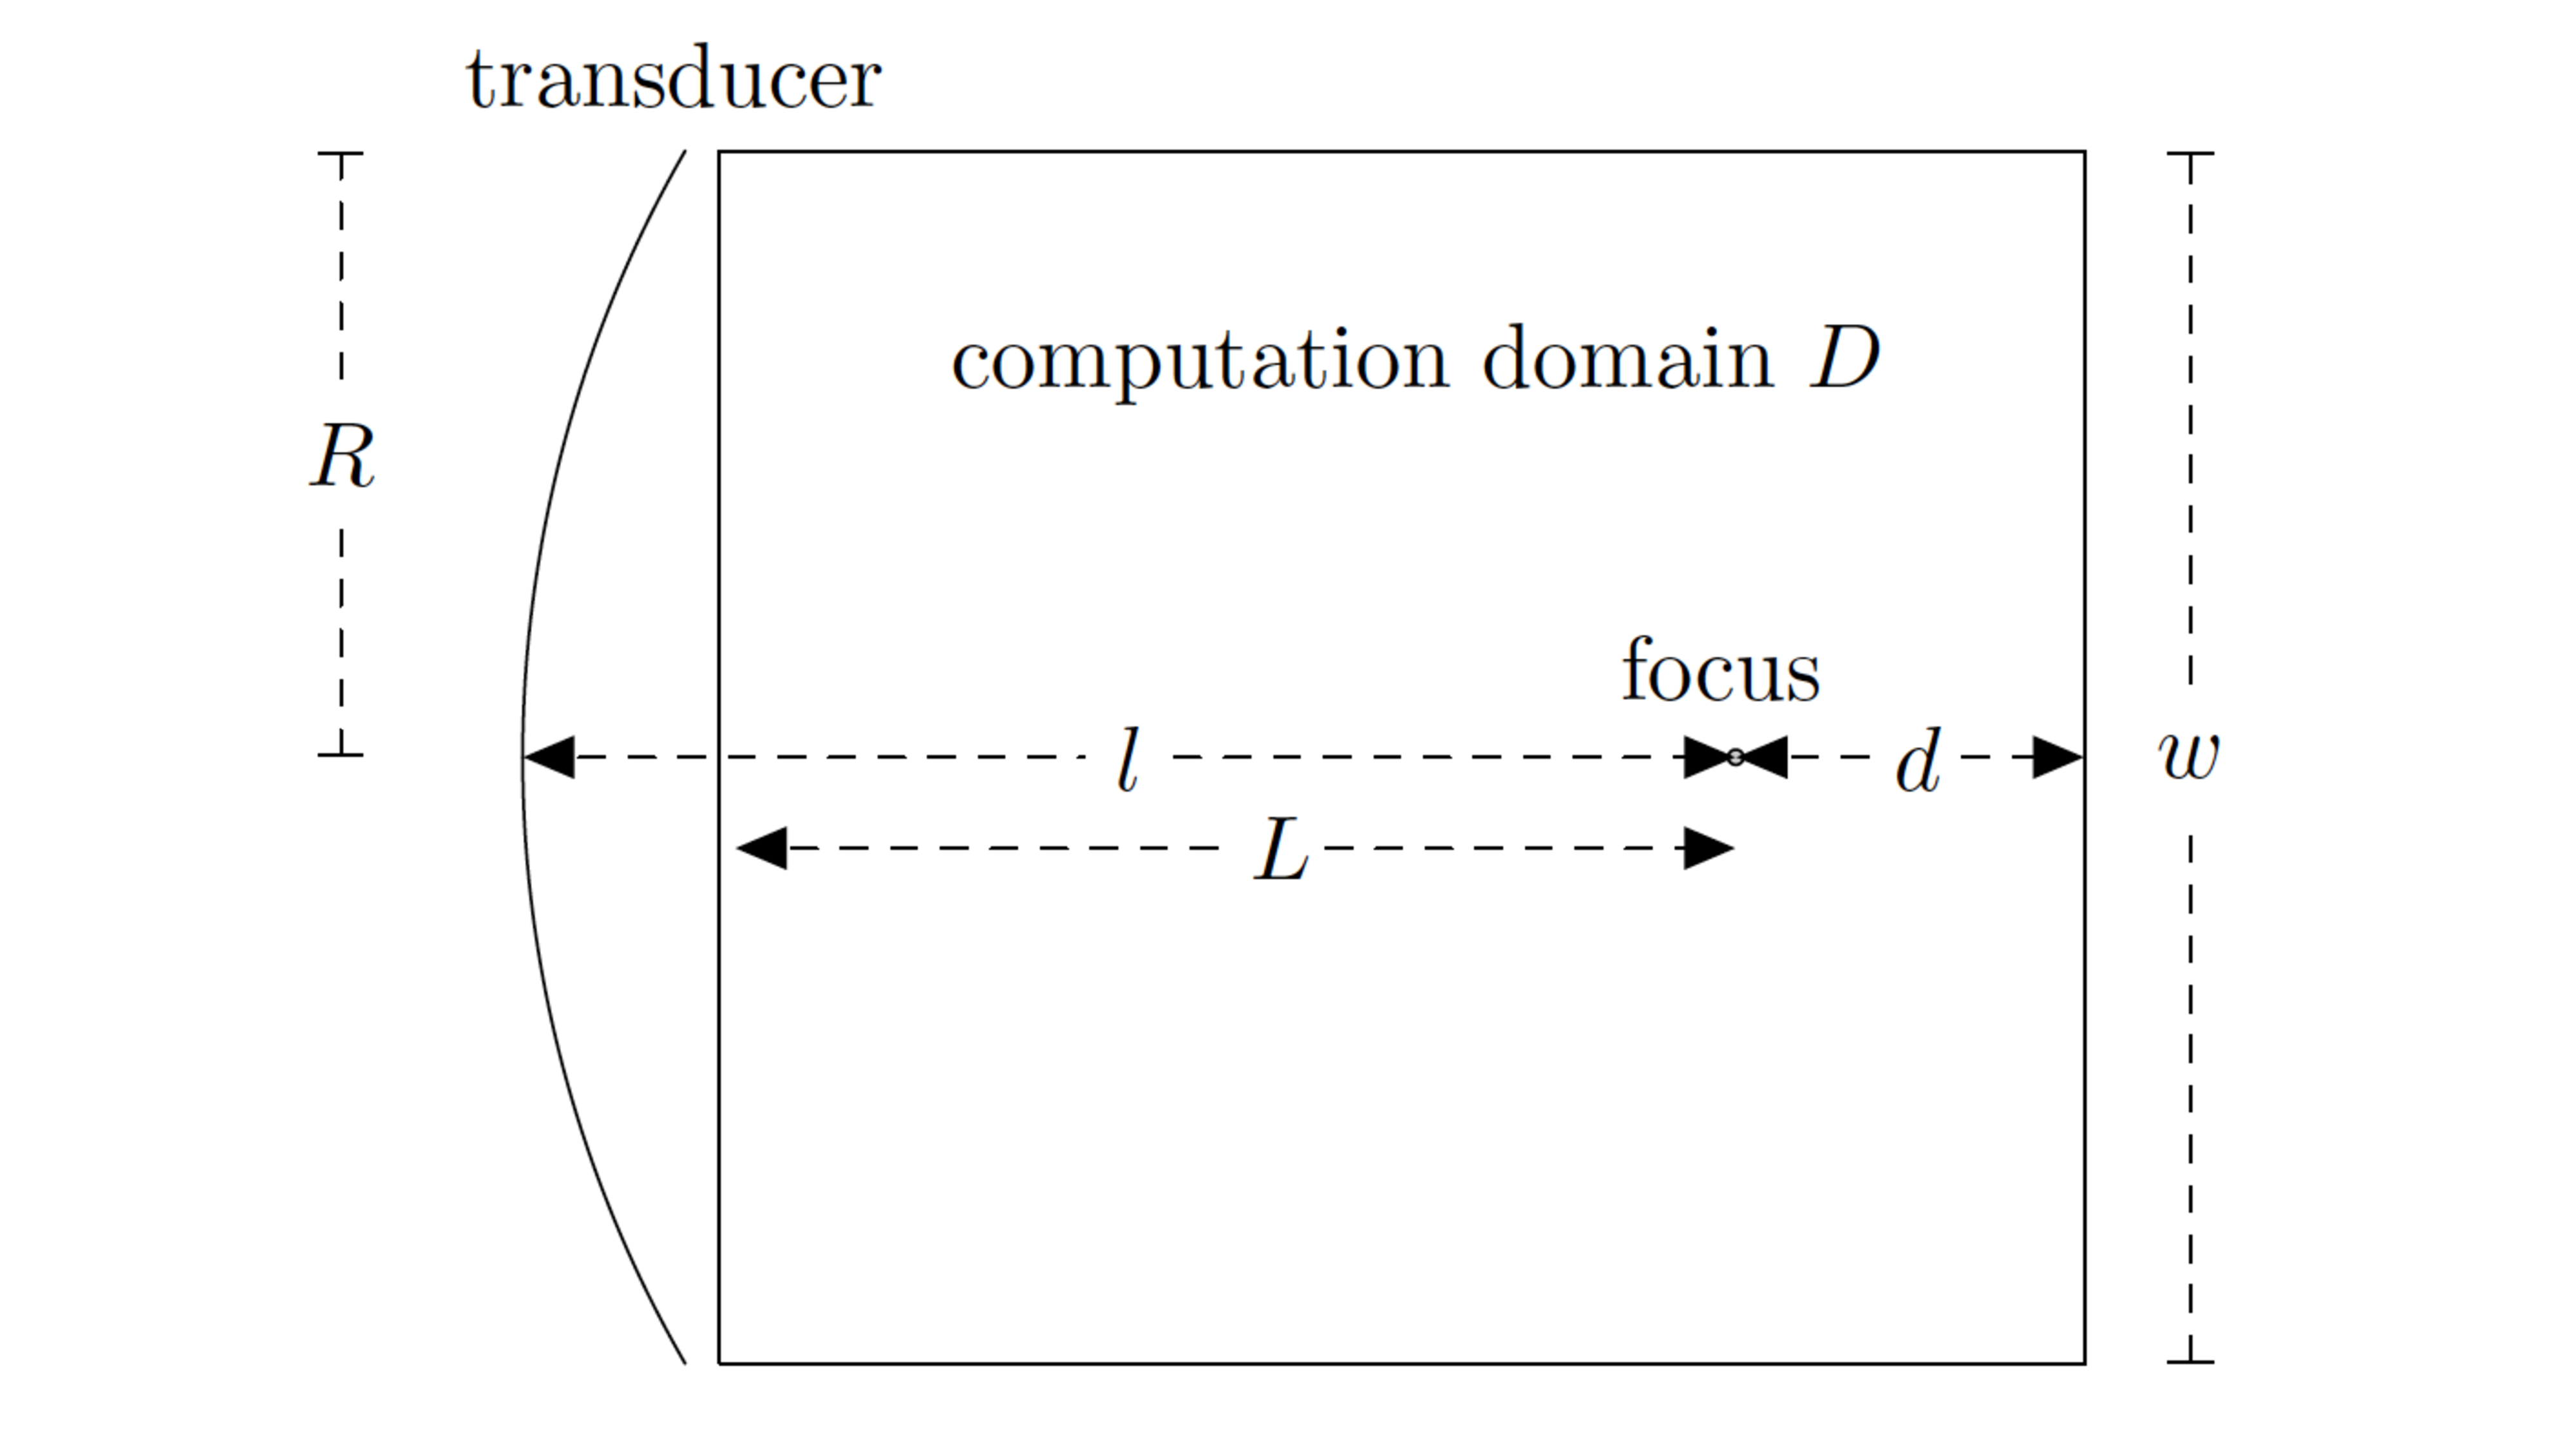
\includegraphics[width=\columnwidth]{Figure1.pdf}
    \caption{Description of a generic computation domain $D$
    with length $L+d$ and width (and depth) $w$.}
    \label{fig:domain_dimensions}
\end{figure}
The domain $D_2$ is defined as 
\begin{equation}
    D_2 = [l-L, l+d] \times [-R, R] \times [-R, R],
    \label{eqn:domain}
\end{equation}
where $d$ is the distance of interest beyond the focus, $l$ is the geometric 
focal length, and $R$ the outer radius (see Fig.~\ref{fig:domain_dimensions}).
The length $L$ is defined as $L = \sqrt{l^2-R^2} - \epsilon$ with $\epsilon$ 
chosen as a small displacement 
from the bowl \red{in order to avoid the possibility of $\bx=\br_i$ in (\ref{eqn:incident_field}),
for which the monopole sources are undefined}; we take $\epsilon = 0.1$mm. 
\red{In this article, we suppose that the region near the focus is of 
primary interest, therefore from a computational point of view, we desire to 
shrink the computation domain to be much shorter and narrower than $L$ and $w$, i.e., 
more localised around the focus, in order to reduce computational load.
The extent to which this shrinking can be done without losing accuracy is the focus 
of sections \ref{sec:results}-\ref{subsec:interpolation}. The values of $L$ and $w$
defined above represent our default computation domain. The value of the distance $d$
depends on the user's interest in the region beyond the focus. In the absence of 
scatterers beyond the focus, the field in this region after the focus will not affect the 
intensity at the focus.}
In the present example, the total radiated power of the
transducer is set as $\Pi_0 = 100$W and the operating frequency is $f_0=1.1$MHz.
\begin{figure}[h!]
    \centering
    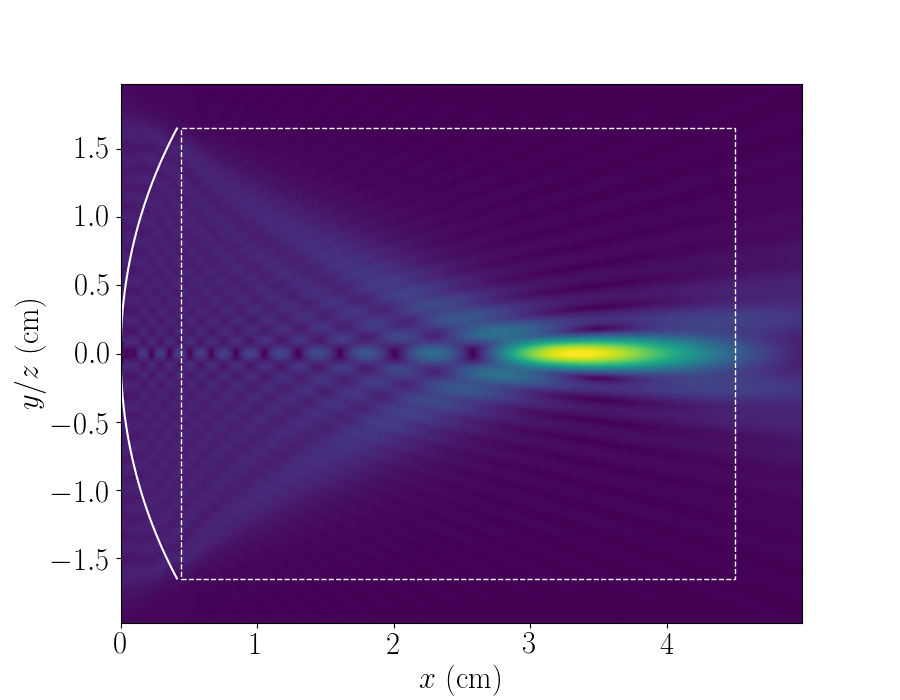
\includegraphics[width=\linewidth]{Figure2}
    \caption{Magnitude of the first harmonic generated by the H131 transducer
    in liver. The bowl transducer is represented by the arc at the far left.
    The dashed white line outlines the computation domain $D_2$ used to compute
    the second harmonic shown in Fig.~\ref{fig:p2_quad}.}
    \label{fig:H131_p1}
\end{figure}

The volume potential in (\ref{eqn:harm2}) is computed using the method outlined 
in Section~\ref{ss:compute_potential} with increasingly refined voxel meshes.
Specifically, we build meshes with voxel dimension $\delta x = \lambda / (2n_w)$,
where $\lambda = c / f_0$ is the fundamental wavelength and $n_w$ is the 
`number of voxels per wavelength'. The factor 2 in the denominator is to account
for the fact that we are computing a field with wavelength $\lambda/2$, i.e.,
the second harmonic. The values of $n_w$ considered are from 4 to 20, and a 
reference solution, denoted $p_2^r$, is computed using $n_w=35$. For each value 
of $n_w$, the relative $L^2$-error of the field $p_2$ along the $x$-axis is 
computed; this is defined as
% \begin{equation}
%     \text{Error} = \frac{\sqrt{\sum_{i=1}^{n_l}(p_2(x_i)-p_2^r(x_i))^2}}
%     {\sqrt{\sum_{i=1}^{n_l}(p_2^r(x_i))^2}}\times 100\%,
% \end{equation}
\begin{equation}
    \text{Error} = \frac{||p_2 - p_2^r||}{||p_2^r||}\times 100\%,
    \label{eqn:error_def}
\end{equation}
where $||\cdot||$ denotes the $L^2$-norm along the $x$-axis, i.e., 
\begin{equation}
    ||p_2|| := \left(\int_{l-L}^{l+d}|p_2(x,0,0)|^2\sd x\right)^{1/2}.
\end{equation}
We approximate the integrals in (\ref{eqn:error_def}) using the midpoint rule
with the mesh nodes of the reference solution, $p_2^r$, being used as the 
quadrature nodes.

\begin{figure}[h!]
    \centering
    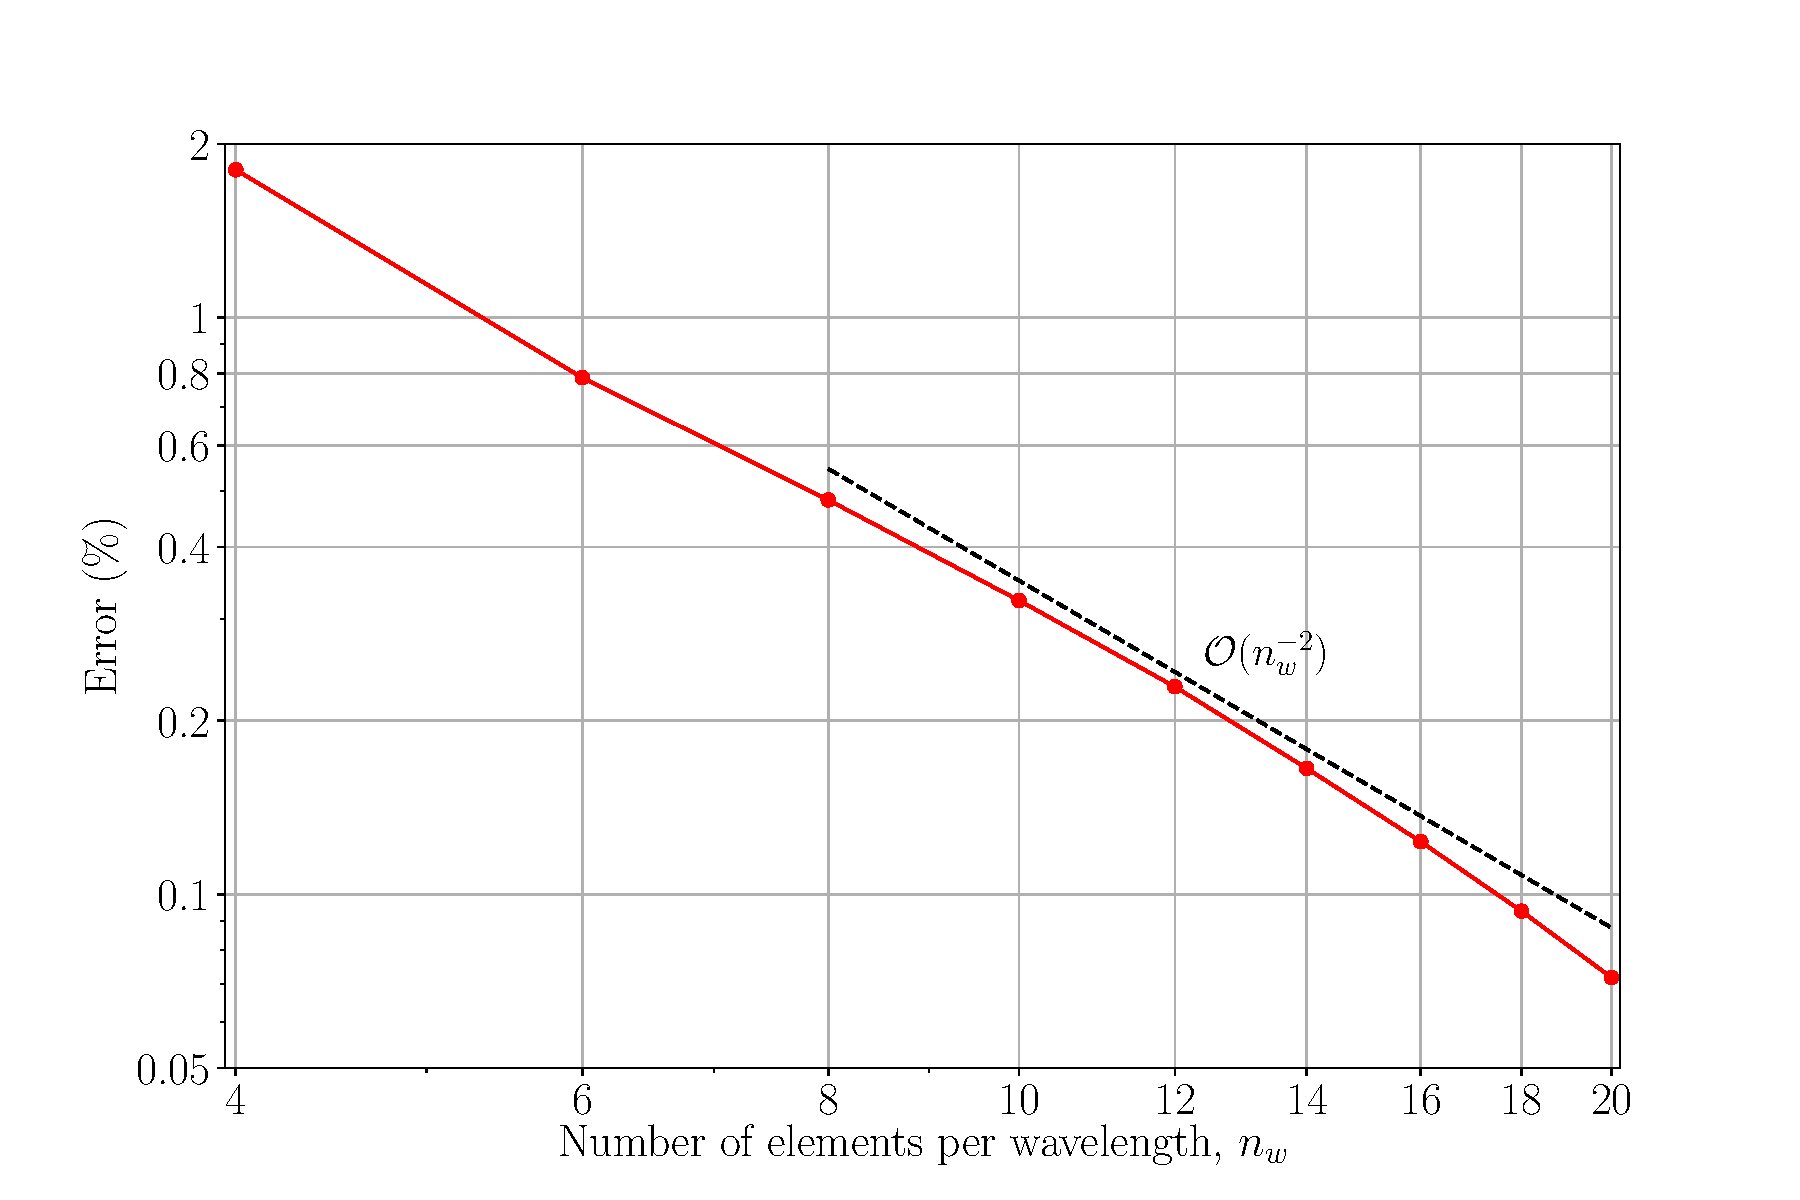
\includegraphics[width=\linewidth]{Figure3.pdf}
    \caption{The convergence of the quadrature rule for the computation of the 
    second harmonic via (\ref{eqn:harm2}). The convergence rate is quadratic
    in $n_w$ and an error of smaller than 1\% is achieved with $n_w>5$.}
    \label{fig:conv_quad}
\end{figure}
The convergence results are shown in Figure~\ref{fig:conv_quad}. As is to be 
expected from the midpoint rule, quadratic convergence is obtained. From the graph 
we can read off that an error smaller than 1\% is achieved with $n_w>5$. 
Therefore we choose to take $n_w=6$ for all harmonics in the experiments in the remainder of the 
article. The approximation to the second harmonic with $n_w=6$ is shown in
Fig.~\ref{fig:p2_quad} and can be seen to be indistinguishable from the
reference solution.
\begin{figure}[h!]
    \centering
    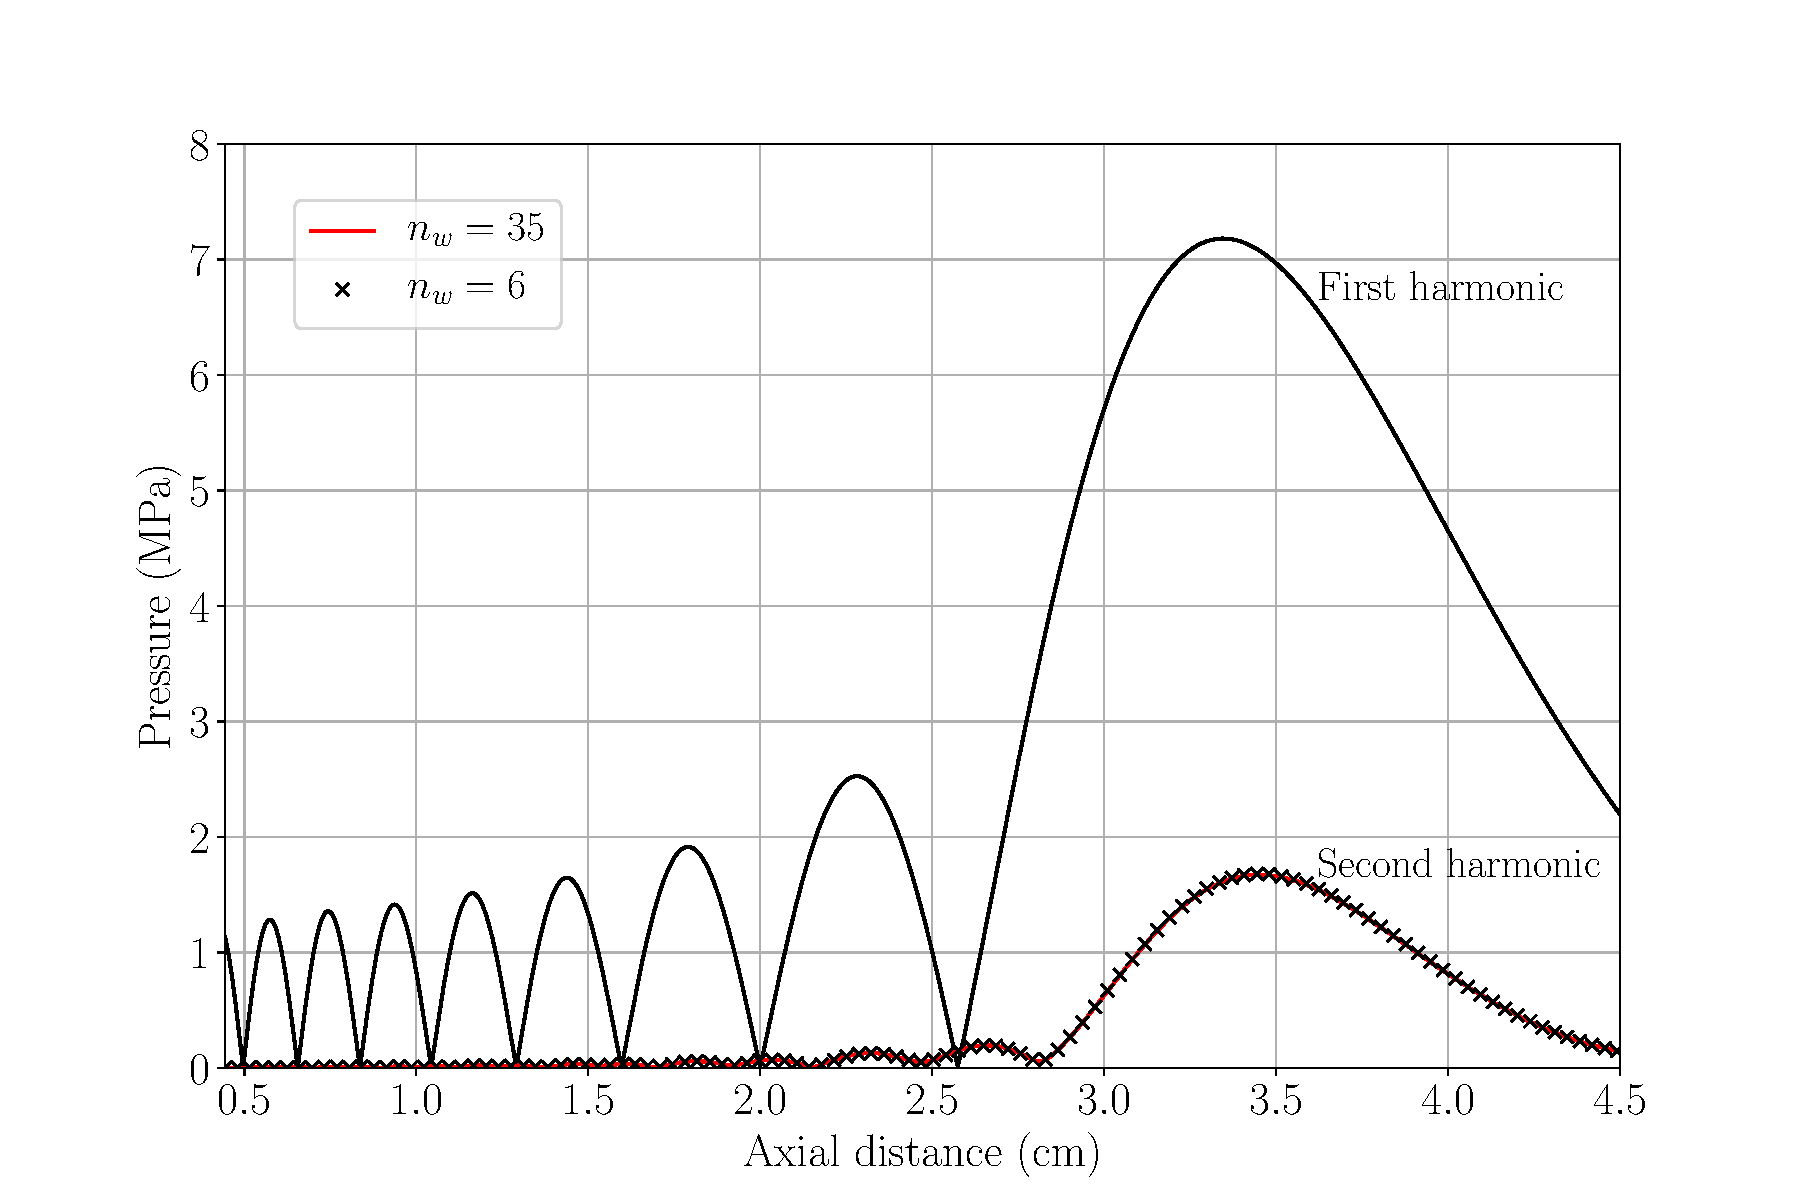
\includegraphics[width=\linewidth]{Figure4.pdf}
    \caption{The first and second harmonics along the $x$-axis for the H131 
    transducer in liver. With 6 voxels per wavelength the approximation to the 
    second harmonic is indistinguishable from the reference solution.}
    \label{fig:p2_quad}
\end{figure}

%%%%%%%%%%%%%%%%%%%%%%%%%%%%%%%%%%%%%%%%%%%%%%%%%%%%%%%%%%%%%%%%%%%%%%%%%%%%%%%%
\section{Validation of numerical scheme}
\label{sec:validation}
To validate our approach for the computation of higher harmonics via the 
evaluation of the volume potentials in (\ref{eqn:harm2})-(\ref{eqn:harm5}), we 
present a qualitative  comparison to approximations obtained using 
\textit{HITU Simulator}~\cite{HITUwebpage}, \red{which we have chosen because of 
its computational efficiency for the axisymmetric problems considered here}. HITU simulator is an open-source \textsc{Matlab}
implementation of the high-order parabolic approximation to the axisymmetric 
Westervelt equation, i.e., the wide-angle Khokhlov-Zabolotkaya-Kuznetsov (WAKZK) equation.
The method is detailed by the author of HITU simulator in \cite{soneson2017extending}.
The assumption of axisymmetry allows the dimension of the problem to be reduced 
by one and hence facilitates rapid simulations. 

We consider two configurations: 
\begin{itemize}
    \item H131 transducer at output power 50W in water;
    \item H101 transducer at output power 100W in liver.
\end{itemize}
\red{These power outputs are chosen since they are relevant to thermal ablation with FUS 
(e.g., \cite{kothapalli2018convenient,ries2010real}) and are sufficiently low to ensure 
that we are in the weakly non-linear setting.}
The first five harmonics along the $x$-axis are shown in 
Fig.~\ref{fig:HITU_comparison_H131} and Fig.~\ref{fig:HITU_comparison_H101}.
In both cases we observe good qualitative agreement with the approximations 
obtained using HITU simulator in the region around the focus, whereas towards the transducer 
the two methods disagree. This is due to the parabolic assumption 
made in the derivation of the WAKZK equation, which is only accurate when 
sufficiently far from the transducer. The volume potential method on the other hand 
approximates solutions to the Westervelt equation so can be taken to be accurate 
in this `near field' region. Indeed, the computation of the first harmonic in 
our approach, as outlined in Section~\ref{subsec:incident}, is equivalent to a Rayleigh 
integral method.
\begin{figure}[h!]
    \centering
    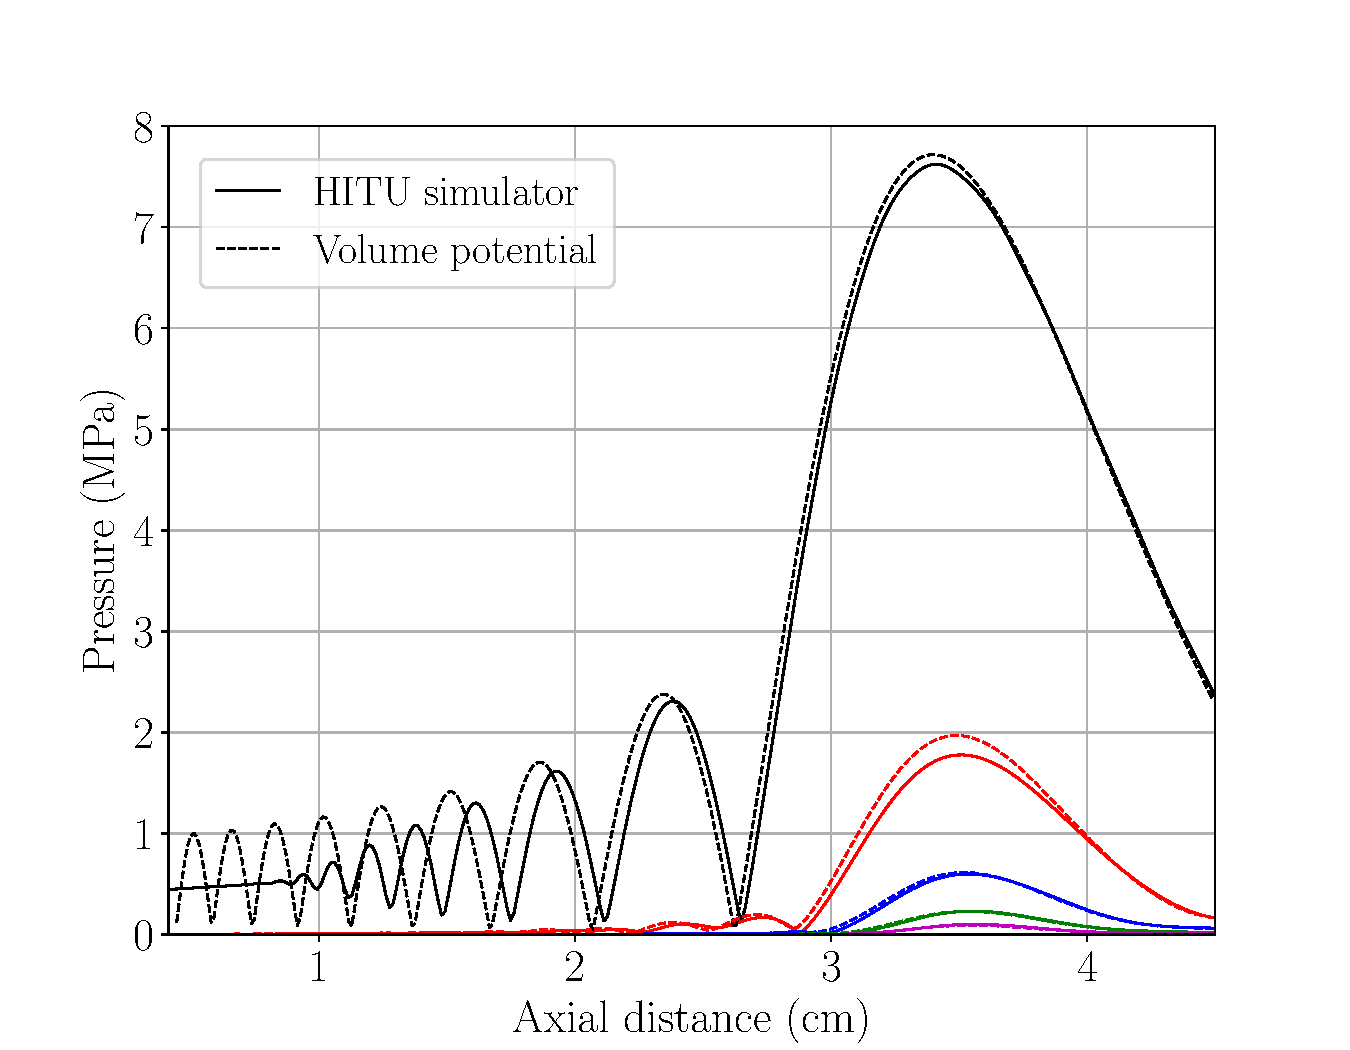
\includegraphics[width=\linewidth]{Figure5.pdf}
    \caption{Comparison of the VIE approach with HITU simulator for the first 
    five harmonics generated by the H131 transducer operating at a power of 50W in water.}
    \label{fig:HITU_comparison_H131}
\end{figure}
\begin{figure}[h!]
    \centering
    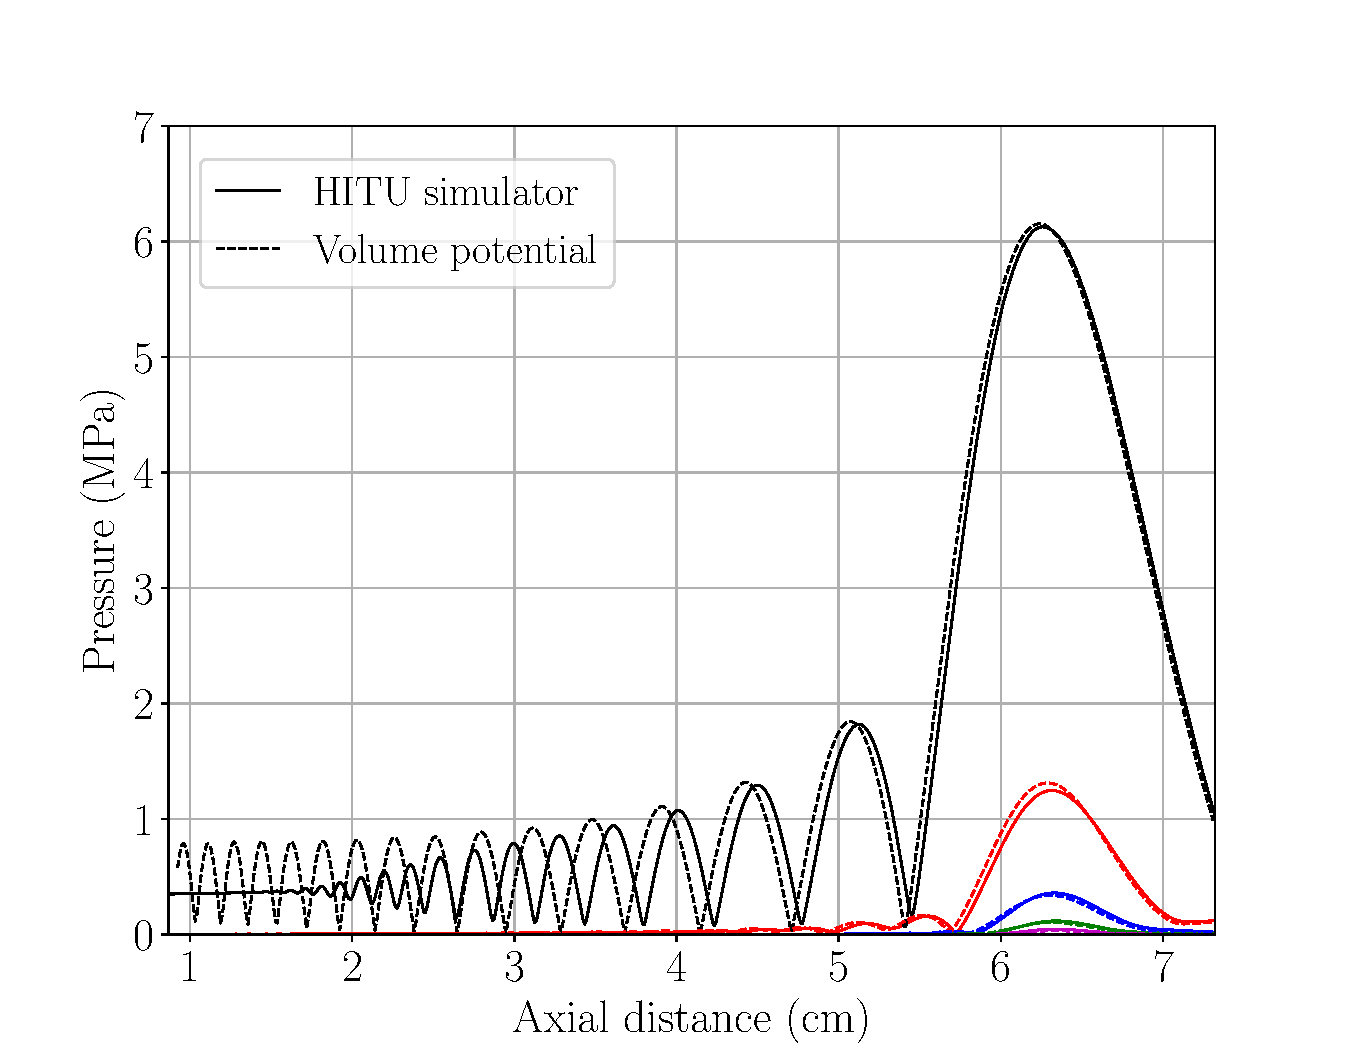
\includegraphics[width=\linewidth]{Figure6.pdf}
    \caption{Comparison of the VIE approach with HITU simulator for the first 
    five harmonics. H101 transducer at power 100W in liver.}
    \label{fig:HITU_comparison_H101}
\end{figure}

\begin{figure*}[ht!]
    \centering
    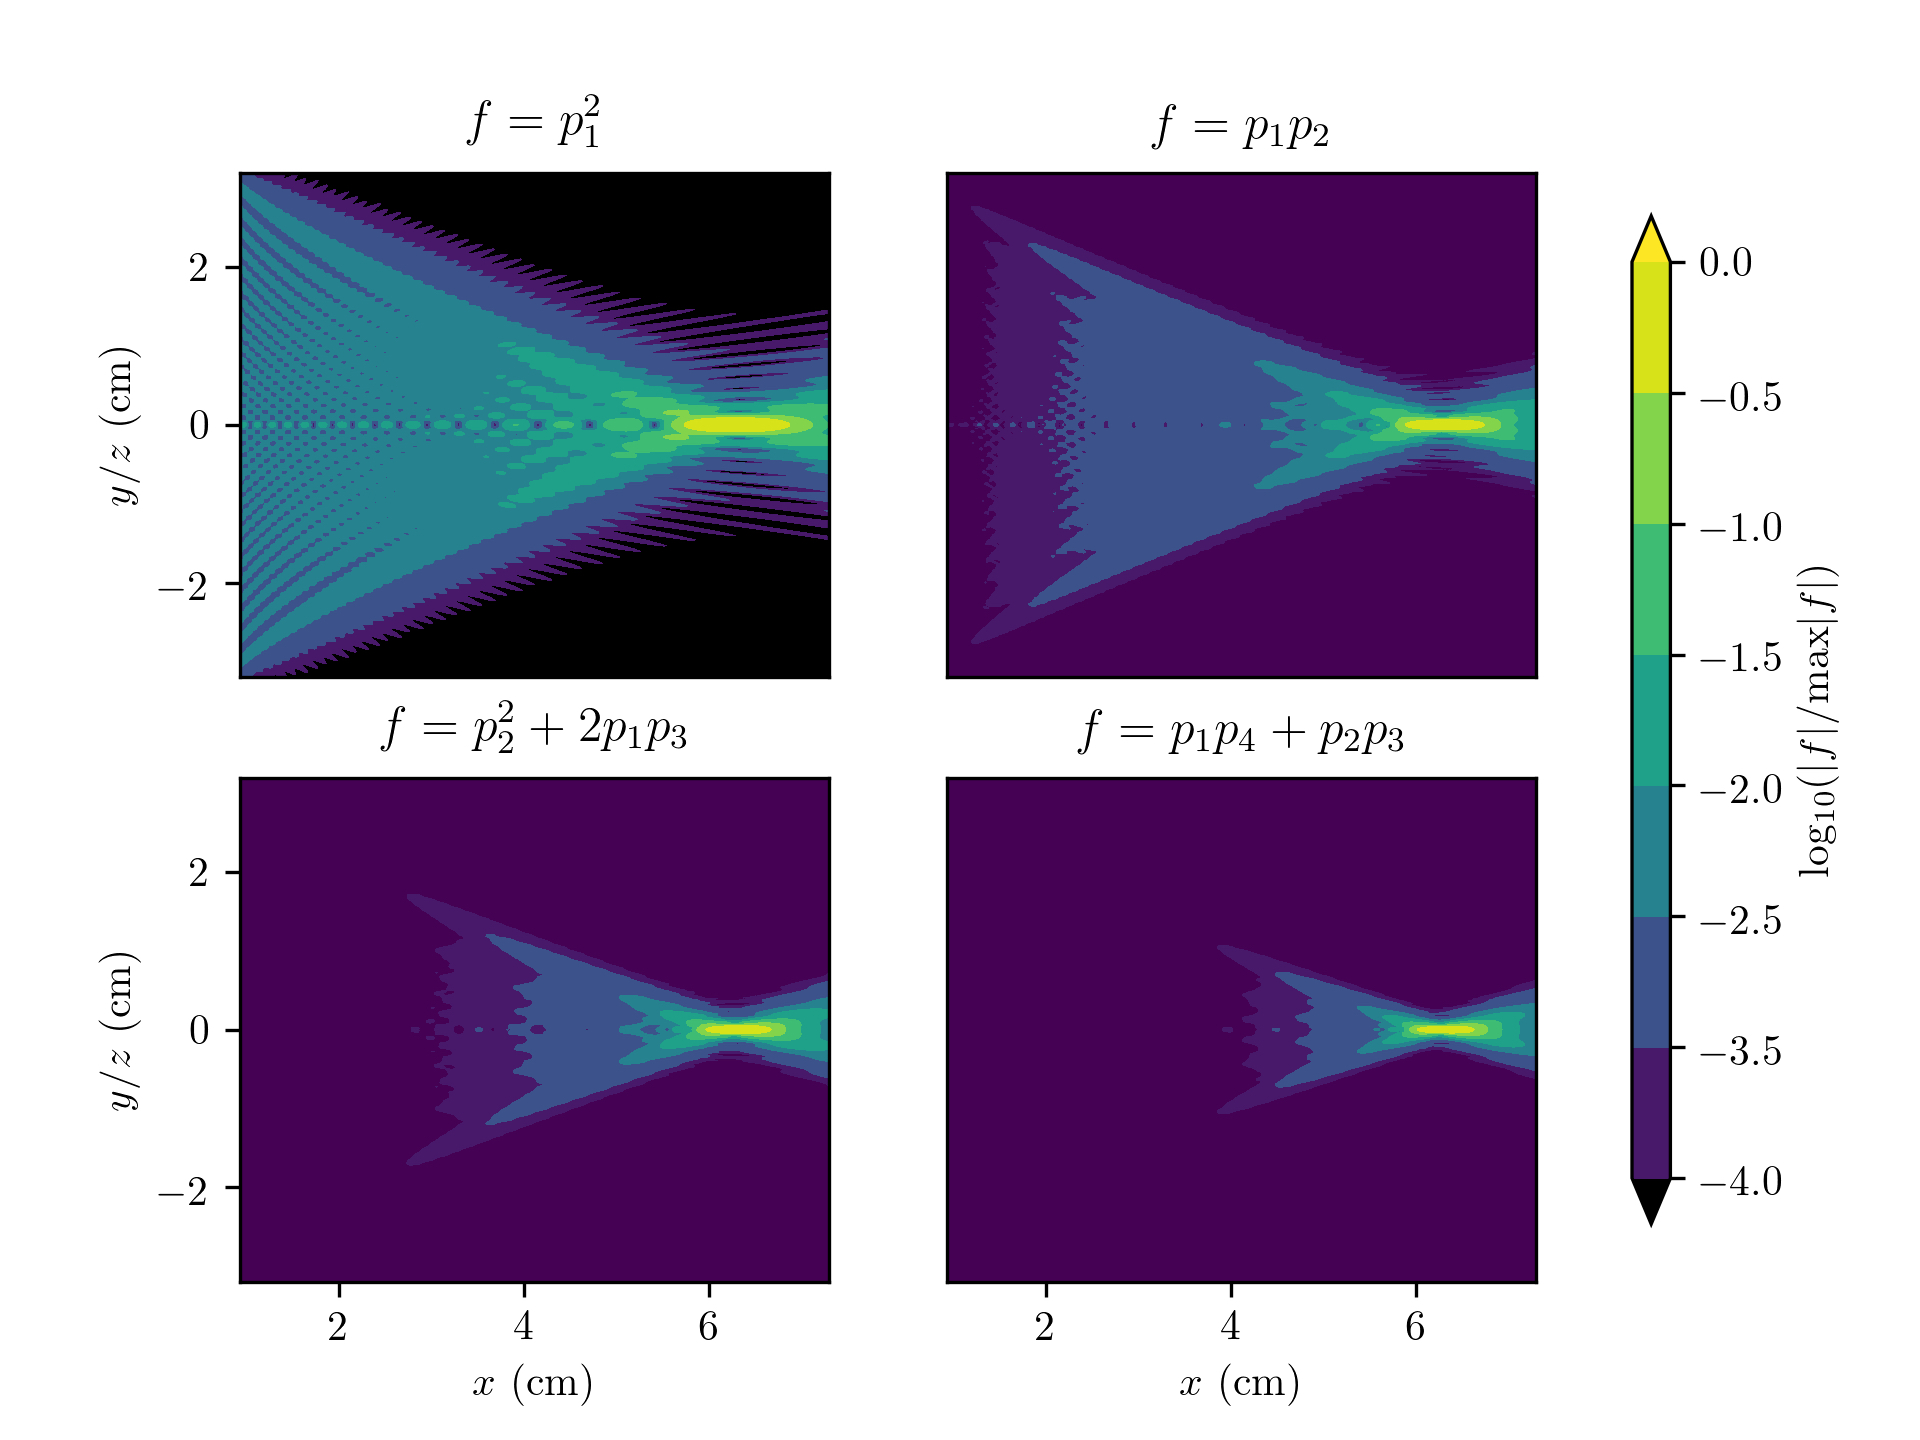
\includegraphics[width=0.95\linewidth]{Figure7}
    \caption{The relative magnitudes of the right-hand side functions 
    $f$ as described in equation (\ref{eqn:RHS}) for the H101 transdcuer in liver,
    at 100W. These plots show how the function to be convolved with the 
    Green's function becomes more localised as the harmonics increase.}
    \label{fig:relative_magnitudes_H101}
\end{figure*} 
We observe that the volume potential method predicts a slightly larger amplitude 
for the first and second harmonics than HITU simulator, \red{which may be because the energy 
flow of the higher harmonics to lower harmonics is neglected in the derivation of 
(\ref{eqn:cascade_2}).} However, the agreement for the third, fourth and 
fifth harmonics is almost perfect. The two examples considered have 
considerably different attenuation power law parameters, thus the strong 
agreement with HITU simulator for both examples demonstrates that the attenuation 
is being handled correctly in the volume potential method.
 
%%%%%%%%%%%%%%%%%%%%%%%%%%%%%%%%%%%%%%%%%%%%%%%%%%%%%%%%%%%%%%%%%%%%%%%%%%%%%%%
\section{Computation domains for successive harmonics}
\label{sec:results}
% In this section we study how the accuracy of higher harmonic computation 
% improves as the size of the computation domain increases. 
In this section we aim to 
determine the amount by which we can restrict the computation domain while 
retaining accurate approximations, and thus enable acceleration of our simulations. 

The main region of interest to practitioners is that around the focus, since 
this is where tissue ablation occurs. Ideally one would compute only 
on that small region. This, however, leads to the second harmonic (and 
thus also the third, fourth, etc.) being poorly approximated since these harmonics
are generated by the accumulation of acoustic energy over distance. So we seek a 
balance between accuracy and computational cost. Here we shall aim to 
keep the error in each harmonic below 1\% (relative to the magnitude of 
the first harmonic) whilst shrinking the integration regions $D_i$ in 
(\ref{eqn:harm2})-(\ref{eqn:harm5}) as much as possible. 

It is important to note that (in this homogeneous setting), the field beyond the 
focal point has no influence on the field in front of it, i.e., the waves propagate
only in the positive $x$-direction. This means that our exploration of domain 
shrinking only applies to the region between the transducer and the focal point.
Beyond the focus we keep the domain length in the $x$-direction fixed. In most
\red{FUS} settings, the practioners are not interested in the field far beyond the 
focal region, therefore the inability to shrink the region beyond the focus does 
not greatly affect the gains achieved from shrinking the computational domain before the focus.

Each of the equations (\ref{eqn:harm2})-(\ref{eqn:harm5}) has the form
\begin{equation}
    p(\bx) = C\int_D G_k(\bx,\by) f(\by) \sd\by,
    \label{eqn:RHS}
\end{equation}
where $f = p_1^2, p_1p_2,\ldots$, $C$ is the appropriate constant, and $k$ is the 
appropriate wavenumber. In order to accurately approximate $p$, the integration 
domain $D$ must enclose the region where the integrand
is non-negligible. Outside of this region, we can discard the contributions. 
The magnitude of the integrand is dictated by the function $f$, which has the 
units of intensity. In order to have
an idea of how localised the different functions $f$ are, we plot them
for a particular example in Fig.~\ref{fig:relative_magnitudes_H101}. The setup considered in the figure 
is the H101 transducer at 100W in liver. The figure shows the magnitudes of $f$
scaled by their maximum values (at the focus) and converted to a log-scale. 
Consider the top-left image: this is the $f$ required for the computation of the 
second harmonic. We can see that the magnitude is significant all the way back 
to the transducer, implying that we must include all this area in the integration 
domain $D$. For the remaining images, corresponding to the third, fourth and 
fifth harmonics, the functions become increasingly more localised in both the 
$x$ and $y/z$ dimensions, suggesting that the required integration domain can
be considerably smaller than that for the second harmonic.

To investigate this more rigorously, we perform convergence tests for each
harmonic as the relevant integration domain $D$ is restricted. That is, we take
the harmonics generated on the domain in (\ref{eqn:domain}) as the reference 
solutions $p_l^r$, $l=2,3,4,5$, and then compute the same harmonics on successively 
smaller domains and compare the approximations to the reference. 
The error of an approximation $p_l$ is computed along the $x$-axis as
\begin{equation}
    \text{Error} = \frac{||p_l-p_l^r||}
    {||p_1^r||}\times 100\%.
\end{equation}
Note that the harmonic
field in the denominator is that of the first harmonic. This is done so that the 
error function incorporates the diminishing size of successive harmonics. For example,
if the fifth harmonic is negligibly small relative to the first harmonic (and so
not worth calculating), the error will reflect this by being very small.

As a measure of the ``localisedness'' of the functions $f$, we use the quantity 
plotted in Fig.~\ref{fig:relative_magnitudes_H101}, which we denote as $Q$:
\begin{equation}
    Q(\bx) := \log_{10}\left(\frac{|f(\bx)|}{\text{max}|f(\bx)|}\right).
    \label{eqn:Q}
\end{equation}
In the convergence tests, the integration domain is chosen as the smallest 
cuboidal domain $D$ such $Q(\bx)<Q_0$ for $\bx\notin D$, where $Q_0$ is a 
given threshold.

The first configuration we \red{perform the convergence experiment for} is the 
H131 transducer in water at an output power of 100W. The convergence for each harmonic is shown in Fig.~\ref{fig:domain_convergence_H131_water}.
We notice that the convergence of the second harmonic drops suddenly 
once the error dips below 1\% -- this is because the computation domain 
is close to the size of the reference domain by this point. This is illustrated 
more clearly in Fig.~\ref{fig:domain_convergence_in_space_H131_water} where the 
same data as in Fig.~\ref{fig:domain_convergence_H131_water} is shown but now 
plotted against the size of the computation domain as a fraction of the reference 
domain, rather than against $Q_0$. \red{By `fraction' of the domain, we mean 
the scaling factor such that the length $L'$ and width $w'$ of the shrunken domain 
are given by 
\[
    L' = \text{fraction}_x\times L,\quad w' = \text{fraction}_{y,z}\times w.    
\]
}

Fig.~\ref{fig:domain_convergence_in_space_H131_water} shows that, to achieve less than 1\% error
in $p_2$, the computation domain must extend all the way to the transducer. 
\begin{figure}[h!]
    \centering
    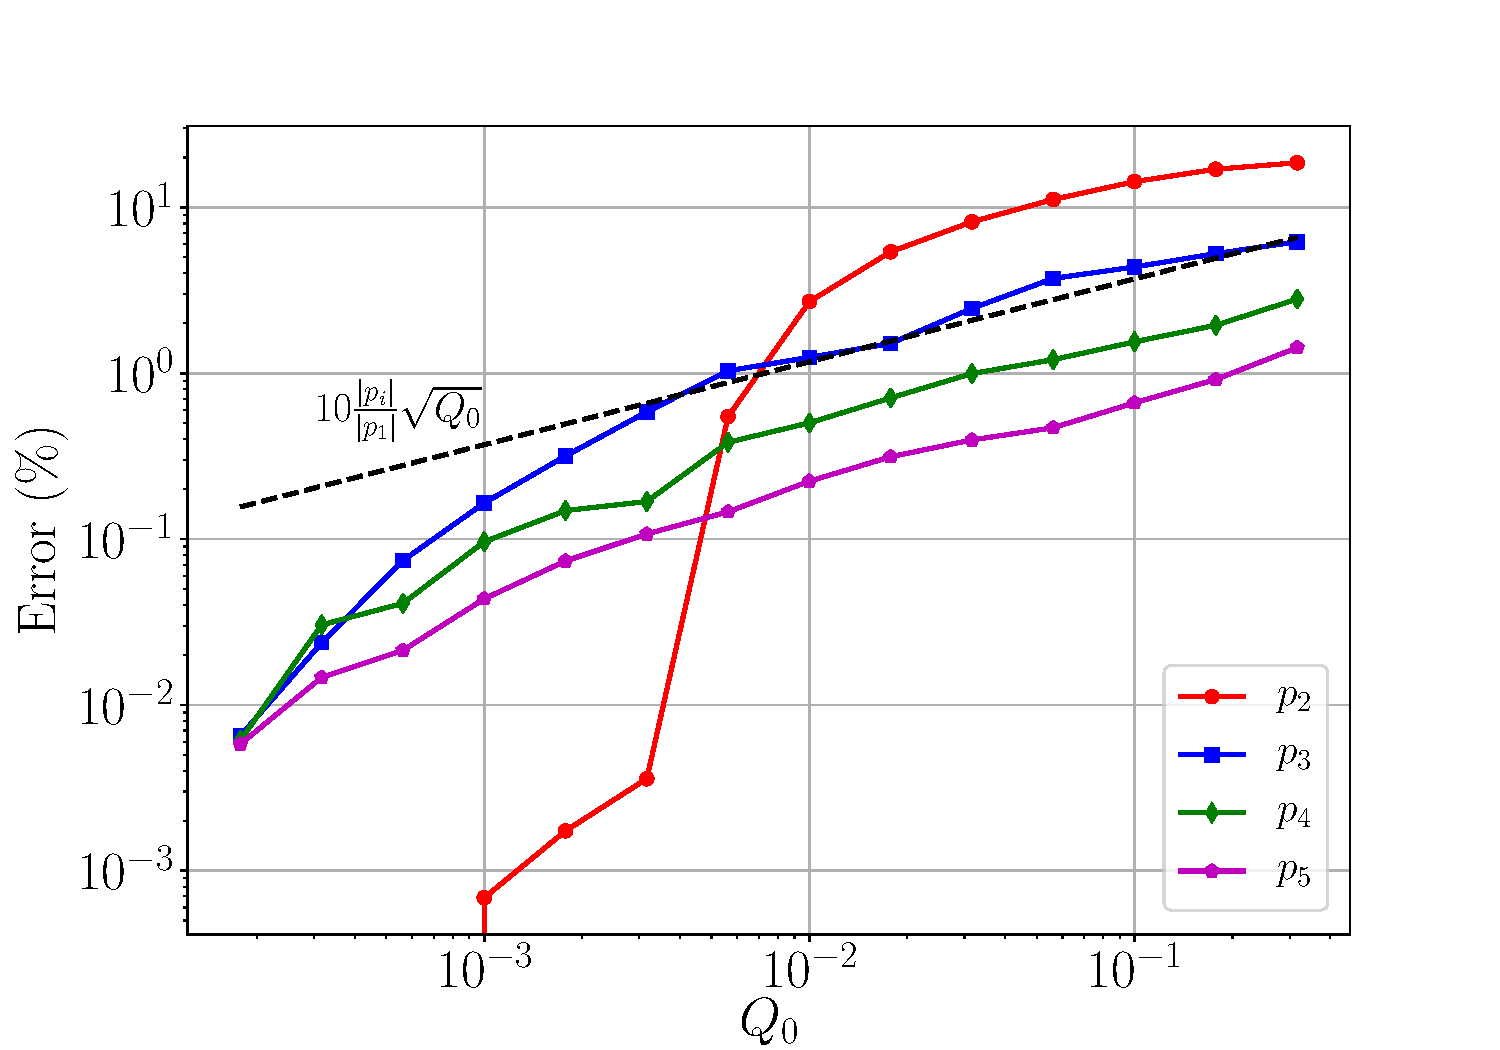
\includegraphics[width=\linewidth]{Figure8}
    \caption{Convergence of the approximations to harmonics $p_i$, $i=2,\ldots,5$
    as the domain of integration $D_i$ for each is adjusted according to the 
    function $Q\geq Q_0$, as defined in (\ref{eqn:Q}). The setup considered here is the H131
    transducer at a power of 100W in water.}
    \label{fig:domain_convergence_H131_water}
\end{figure}
For the higher harmonics, however, a different trend is evident. In Fig.~\ref{fig:domain_convergence_H131_water}
we observe that the error curves for $p_3,p_4,p_5$ each have the approximate behaviour
\begin{equation}
    \text{Error}(p_i) \approx 10\frac{||p_i||}{||p_1||}\sqrt{Q_0},\quad i=3,4,5,
    \label{eqn:trend}
\end{equation}
where $||\cdot||$ represents the $L^2$-norm. Although an interesting observation, 
the utility of the relationship (\ref{eqn:trend}) for dictating an appropriate 
computation domain for $p_i$ is not immediately apparent, since it requires the 
computation of $||p_i||$ before $p_i$ has been computed. Determining an \emph{a priori} 
approximation for $||p_i||$ to make use of (\ref{eqn:trend}) would be a useful
endeavour, however we do not undertake such a task in this article. Rather we 
seek to develop an approximate rule of thumb for choosing sensibly-sized computation domains 
for the harmonics. To this end, it is more straightforward to consider the 
convergence of the approximations in terms of physical distance, as is done in 
Fig.~\ref{fig:domain_convergence_in_space_H131_water} and Tab.~\ref{tab:convergence_domain}.
\begin{figure}[h!]
    \centering
    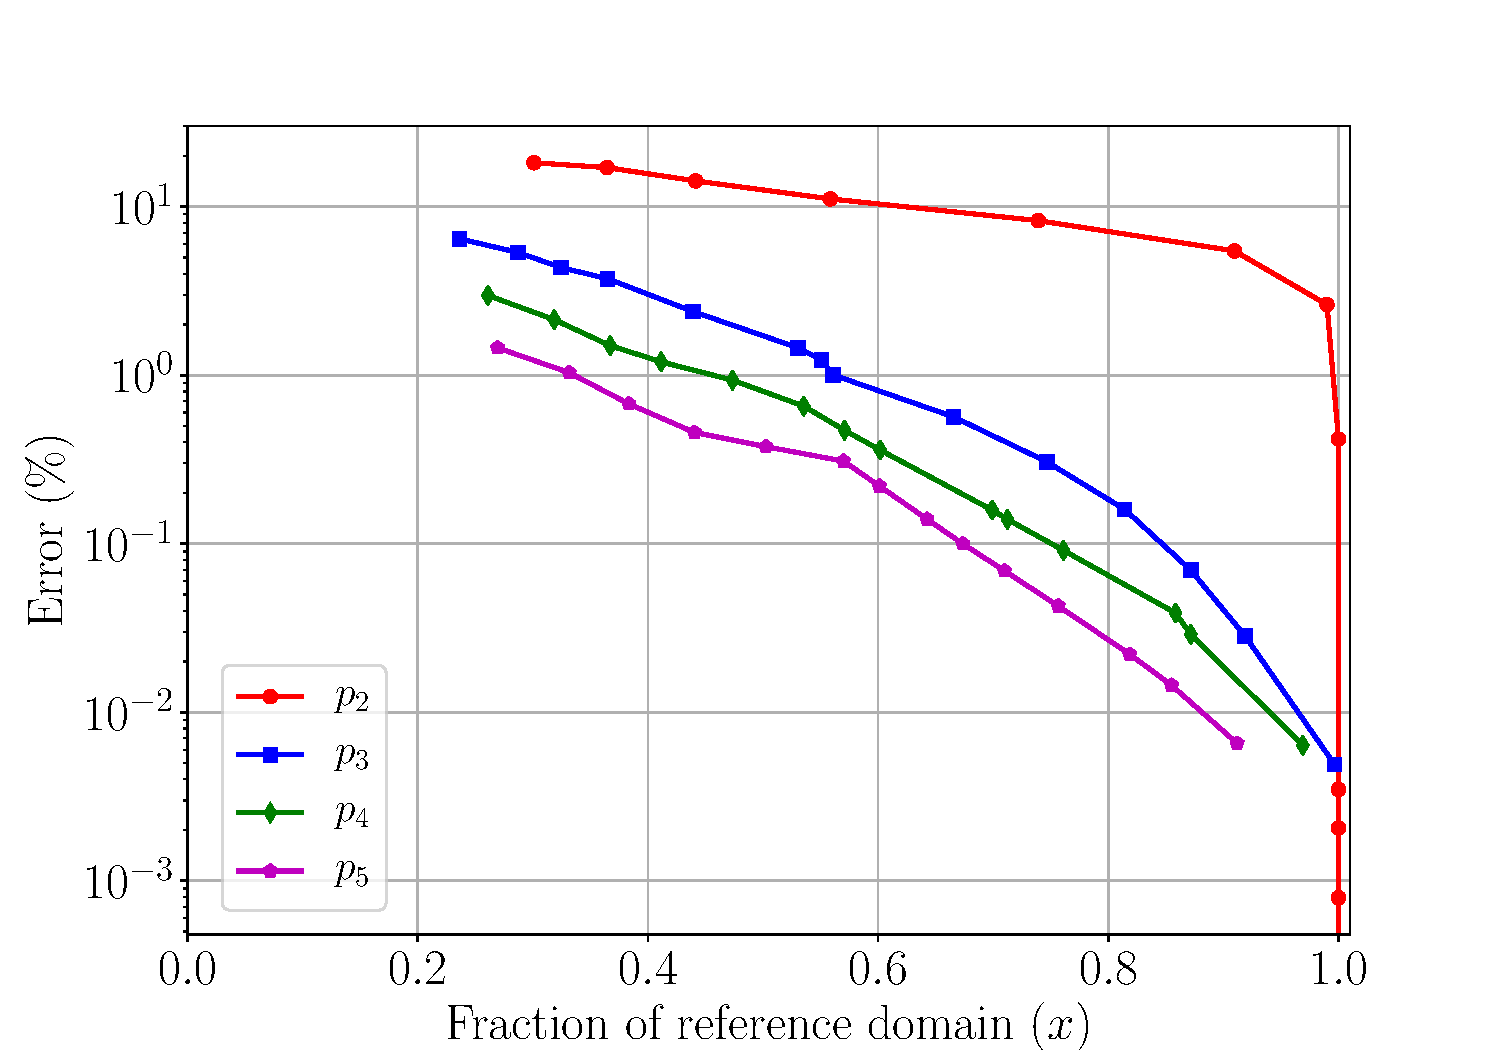
\includegraphics[width=\linewidth]{Figure9}
    \caption{Convergence for H131 transducer at 100W in water, as in Fig.~\ref{fig:domain_convergence_H131_water}.
    The error is plotted against the fraction of the total domain in the $x$-direction.
    This demonstrates that, to achieve an error smaller than 1\%, the computation 
    domains can be contracted significantly in the $x$-direction for harmonics higher than the second.}
    \label{fig:domain_convergence_in_space_H131_water}
\end{figure}

By looking at the 1\% error line in Fig.~\ref{fig:domain_convergence_in_space_H131_water},
it is possible to read off the size of the domains as fractions of the reference
domain. The precise values are reported in Tab.~\ref{tab:convergence_domain}.
A nested series of domains constructed according to this specification is shown 
in Fig.~\ref{fig:H131_water_subdomains}. Let us elaborate on the potential 
computational gain achieved using these nested domains compared to computing 
all harmonics on the reference domain.

The reference domain for the H131 transducer in water has dimensions 
$[4.1\text{cm},3.3\text{cm},3.3\text{cm}]$ and is discretised into voxels of dimension 
$\delta x = \lambda_5/6\approx \red{45.1\mu}$m, i.e., fine enough to 
resolve the highest harmonic of interest. This mesh has 
$901\cdot 732\cdot 732\approx 4.8\times 10^8$ voxels for the computation of all 
the harmonics. Using the nested domains built according to the specifications in 
Tab.~\ref{tab:convergence_domain}, we obtain a mesh for $p_2$ with dimensions
$[4.1, 2.4, 2.4]$cm, which is discretised into voxels of dimension 
$\delta x = \lambda_2/6\approx \red{113\mu}$m. This mesh has 
$360\cdot 211\cdot 211\approx 1.6\times 10^7$ voxels, which is a factor of 
30 smaller than the reference mesh. \red{The meshes for the computation of $p_3, p_4$
and $p_5$ have $1.22\times10^7, 6.1\times10^6$ and $4.5\times10^6$ voxels, respectively.
Thus the total number of voxels required for all harmonics is $4\times4.8\times 10^8=19\times 10^8$ for 
the single mesh approach and $3.9\times 10^7$ for the nested meshing (summing over 
voxels in each of the four meshes). Hence we achieve close to a factor 50 reduction in computational load.}

% The meshes for the higher harmonics have 
% even fewer voxels and so overall we achieve more than a factor 30 reduction in 
% computational load compared to computing all harmonics on the reference mesh.
\begin{table}[h!]
    \centering
    \begin{tabular}{c | c  c  c  c  c}
        \hline\hline
             &     & $p_2$ & $p_3$ & $p_4$ & $p_5$ \\
        \hline
        H131 water & $x$   & 1 & 0.67 & 0.47 & 0.38 \\
        100W & $y/z$ & 0.74 & 0.39 & 0.20 & 0.13 \\
        \hline
        H131 water & $x$   & 1 & 0.67 & 0.58 & 0.52 \\
        150W & $y/z$ & 0.71 & 0.40 & 0.39 & 0.21 \\
        \hline
        H131 liver & $x$   & 1 & 0.56 & 0.25 & 0.26 \\
        100W & $y/z$ & 0.90 & 0.20 & 0.05 & 0.06 \\
        % \hline
        % H101 water & $x$   & 1 & 0.47 & 0.27 & 0.16 \\
        % 100W & $y/z$ & 0.95 & 0.37 & 0.28 & 0.23 \\
        \hline
        Rule of & $x$  &  1 & 0.75 & 0.65 & 0.61 \\
        thumb   & $y/z$ & 1 & 0.67 & 0.5 & 0.4
    \end{tabular}
    \caption{Sizes of domains required to achieve less than 1\% error for each 
    harmonic as fractions of the reference domain (\ref{eqn:domain}). Since all 
    domains are boxes, the fractions of the distances in the $x$ and $y/z$ directions 
    are provided.}
    \label{tab:convergence_domain}
\end{table}

This improvement is impressive, however it is easily seen in Tab.~\ref{tab:convergence_domain}
that this particular domain scaling does not apply to all transducer and material
configurations. Therefore, we decide upon a simple rule of thumb for designing
the separate computational domains that leads to domains greater than or 
equal to those given in Tab.~\ref{tab:convergence_domain}. Therefore, the errors 
incurred in using these domains will be even smaller than those obtained when using
the ideal domains specified in the table.

A desirable rule for domain sizes would be the following:
\begin{quoting}
    Let $[L+d, w, w]$ be the dimensions of domain $D_2$ (see Fig.~\ref{fig:domain_dimensions})
    for harmonic $p_2$, with corresponding wavelength $\lambda_2$. Then 
    choose the dimensions of domain $D_{i}$, $i>2$, as 
    $[\frac{\lambda_i}{\lambda_2}L+d, \frac{\lambda_i}{\lambda_2}w, \frac{\lambda_i}{\lambda_2}w]$. That is,
    the domain is scaled according to the wavelength of the harmonic being considered.
\end{quoting}
With this rule for creating the domains, we observe that the number of voxels in 
each mesh will almost be the same, save for a slight increase due to the 
fact that the distance $d$ is not being scaled. This amounts to a reduction in 
the overall number of DOF by a factor of approximately $(n/2)^3$ (in fact, slightly
lower than this due to the unscaled portion of length $d$), where $n$ 
is the number of harmonics being computed.


\begin{figure}[h!]
    \centering
    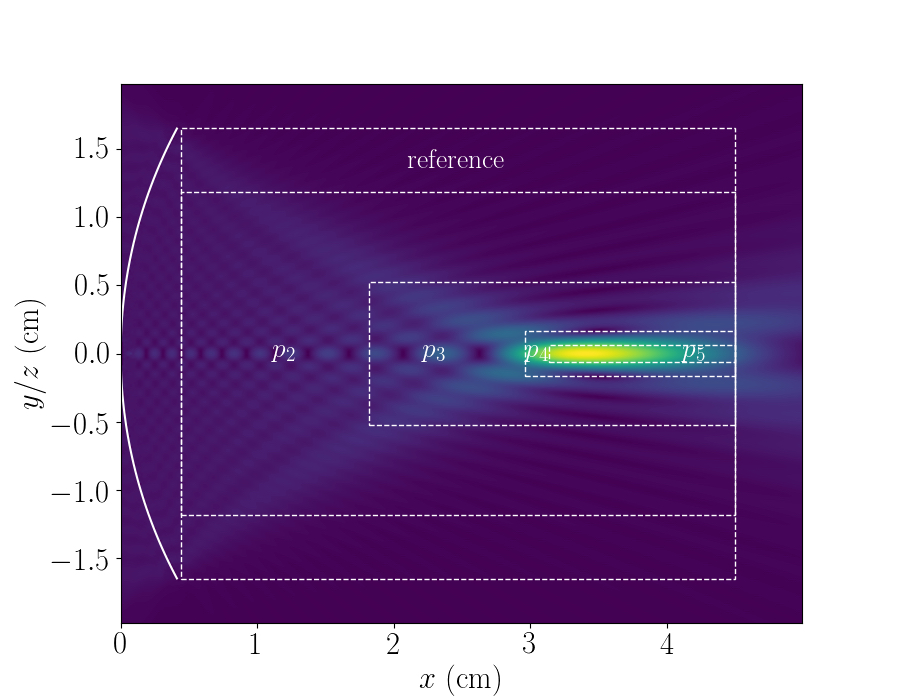
\includegraphics[width=\linewidth]{Figure10}
    \caption{Nested domains for the computation of successive harmonics while
    keeping relative error below 1\%, for the H131 transducer operating at 100W 
    in water. The domain used to compute the reference 
    solution is in (\ref{eqn:domain}).}
    \label{fig:H131_water_subdomains}
\end{figure}  

In the next section, we outline an algorithm for evaluating the volume potentials 
over a set of nested domains constructed according to the rule of thumb proposed above.


%%%%%%%%%%%%%%%%%%%%%%%%%%%%%%%%%%%%%%%%%%%%%%%%%%%%%%%%%%%%%%%%%%%%%%%%%%%%%
\begin{table*}[ht!]
    \centering
    \begin{tabular}{c  c  c  c  c c}
        \hline\hline
           &  N$^\circ$ voxels & Meshing & Interpolation & Evaluate $G_{k_i}$ & Compute $p_i$\\
        \hline
        $p_2$ & $1.86\times10^8$ & 26.1s & 24m30s & 4m54s & 3m48s \\
        $p_3$ & $2.01\times10^8$ & 22.2s & 3m9s & 5m14s & 4m9s\\
        $p_4$ & $2.15\times10^8$ & 23.9s & 5m50s & 5m27s   & 4m8s   \\
        $p_5$ & $2.30\times10^8$ & 25.5s & 7m12s & 6m7s   & 7m5s \\
        \hline\hline
    \end{tabular}
    \caption{Performance details for the volume potential approach on nested 
    meshes with a resolution of six voxels per wavelength (for each harmonic). 
    The configuration considered is the H101 transducer operating at 100W in water.
    Total time taken 1h23m11s.}
    \label{tab:performance}
\end{table*}

%%%%%%%%%%%%%%%%%%%%%%%%%%%%%%%%%%%%%%%%%%%%%%%%%%%%%%%%%%%%%%%%%%%%%%%%%%%
\section{Volume potentials on nested meshes}
\label{subsec:interpolation}
To demonstrate the effectiveness of the volume potential evaluation on nested meshes, 
we present some final results detailing the computational performance of this 
approach. First we outline the algorithm for computing the first $n$ harmonics:
\begin{algorithmic}
    \For {$i=2\rightarrow n$}
    \begin{enumerate}
        \item Create domain $D_i$ for $p_i$ and voxel mesh $\mathcal{V}(D_i)$
        \item Assemble components for integration (\ref{eqn:quad}):
            \begin{enumerate}
                \item Evaluate/interpolate $p_{i-1},p_{i-2},\ldots,p_1$ at voxel centres in $\mathcal{V}(D_i)$
                \item Evaluate integral of Green's function $G_{k_i}$ over each voxel
            \end{enumerate}
        \item Compute $p_i$ via appropriate equation in (\ref{eqn:harm2})--(\ref{eqn:harm5})
    \end{enumerate}
    \EndFor
\end{algorithmic}
Note that in the above algorithm, for $p_2$, the pressure field $p_1$ is evaluated
over the voxel mesh $\mathcal{V}(D_2)$ as described in Section~\ref{subsec:incident}. 
Whereas for later harmonics we perform interpolation of the earlier harmonics down
onto the new mesh. In this work we have used linear interpolation, however if 
higher accuracy is required, we recommend quadratic interpolation (albeit at a 
higher computational cost). The second and third step each contain applications of the 
FFT: for the circulant embedding of the Green's function in step 2
(see, e.g., \cite{groth2020accelerating}) and to perform the convolution 
required in the quadrature rule (\ref{eqn:quad}) in step 3.
These FFTs are performed using the Python wrapper `pyfftw' to the FFTW 
library~\cite{FFTW05}. 

As an example, we consider the H101 transducer operating at 100W in water
run on a workstation with two sockets, each containing a 14-core Xeon E5-2690 
v4 CPU, each supporting hyper-threading with two threads, and hence a total 
number of 56 threads. The total amount of RAM available on this machine is 
approximately 270GB, which is ample for the problems considered here.
The first five harmonics along the $x$-axis are shown in 
Fig.~\ref{fig:HITU_comparison_H101_water}, along with the approximation obtained 
with HITU simulator; again we see that the volume potential approach predicts a 
larger peak in the second harmonic but in general a good qualitative agreement
is observed.

To get a feel for the performance of our approach (of evaluating the volume potentials
on nested meshes designed according to our proposed rule of thumb), the cost of each 
step in the above algorithm is detailed in Tab.~\ref{tab:performance}. The 
largest mesh has 230 million voxels, as compared to 2.9 billion voxels without 
nested meshing. This represents a large saving, in both time and memory. The 
most expensive step reported in Tab.~\ref{tab:performance} is the evaluation of 
the first harmonic $p_1$ on $\mathcal{V}(D_2)$. This process was described in 
Section~\ref{subsec:incident} and has complexity $\mathcal{O}(n_e N)$, where $n_e$ is 
number of points used to discretise the surface of the transducer and $N$ is the 
number of voxels.
Since we take $n_e=4096$, this is a rather expensive procedure, even when parallelised
over 56 threads. Therefore a transducer model using far fewer elements and/or a machine
with more threads will lead to a large reduction in computation time for this step.
Linear interpolation is computed efficiently using the scipy~\cite{jones2001scipy} \verb!RegularGridInterpolator!
command. The evaluation of $G_{k_i}$ consists of a parallelised loop over the 
$N$ voxels and then an FFT of a three-dimensional complex-valued array of size $(2N_x,2N_y,2N_z)$,
where $N_x,N_y,N_z$ are the number of voxels in each dimension. Then the computation
of $p_i$ consists of one forward and one inverse FFT of an array of size $(2N_x,2N_y,2N_z)$.
The FFTs take advantage of multithreading, therefore can be easily accelerated 
through the use of more cores. Furthermore, it seems likely that optimising the 
FFT routine for the particular setting and using the FFTW C++ library directly 
will lead to further acceleration. Nevertheless, the current implementation yields fast and accurate predictions of 
the first five harmonics (in the cases considered).

\begin{figure}[h!]
    \centering
    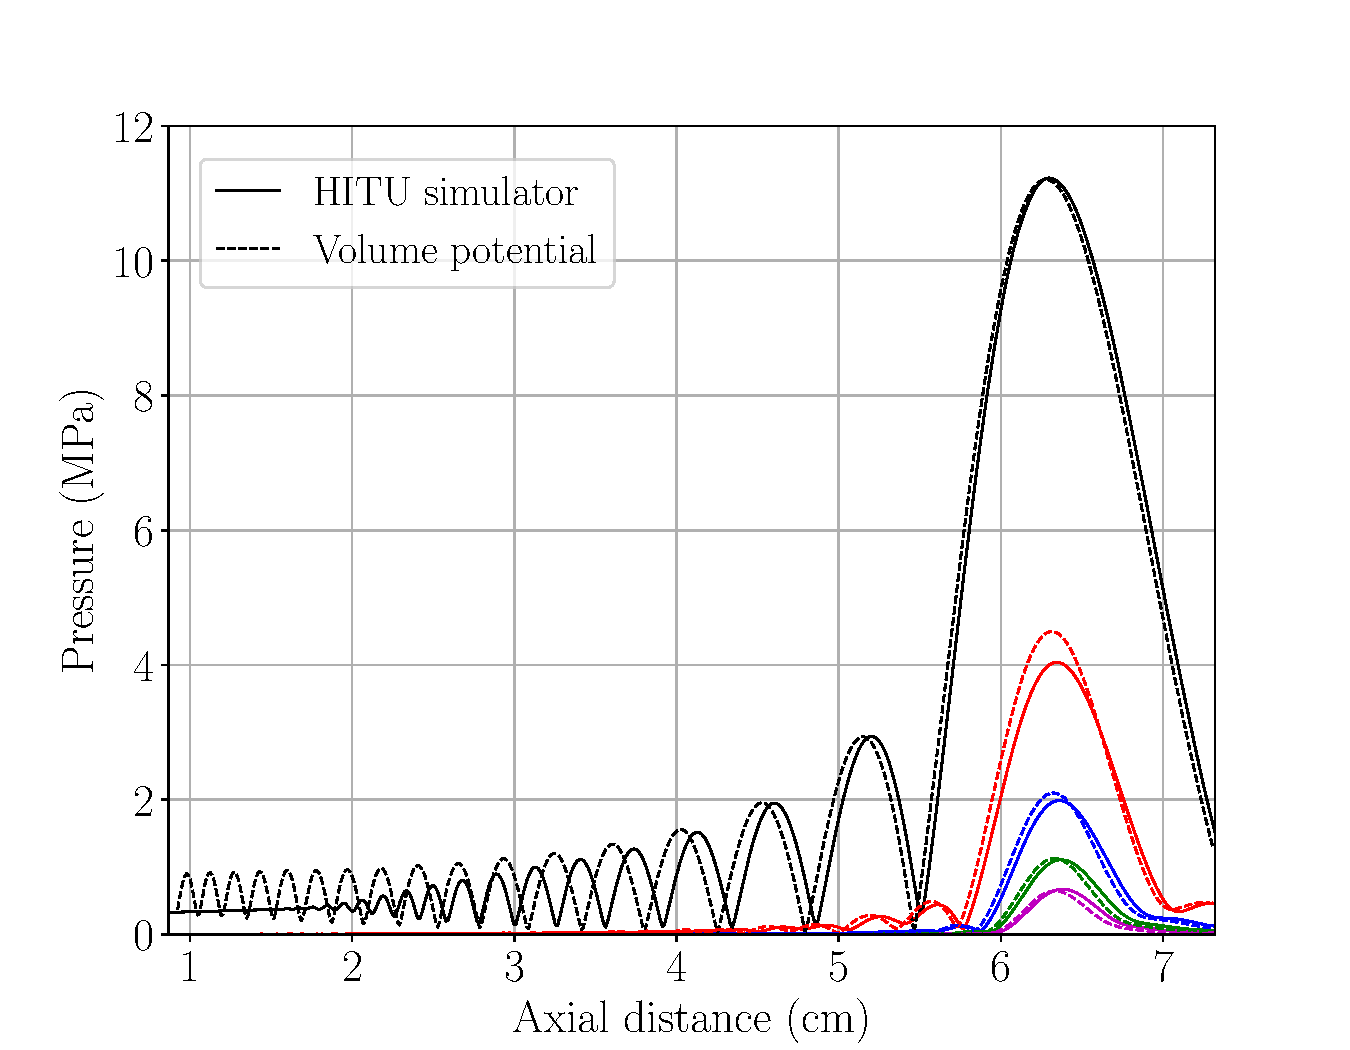
\includegraphics[width=\linewidth]{Figure11}
    \caption{The on-axis absolute pressure field for the first five harmonics generated 
    by the H101 transducer at 100W in water, as 
    computed using the volume potential approach on nested domains, designed to 
    keep the relative error below 1\%. The approximation obtained using the HITU
    simulator is provided for comparison.}
    \label{fig:HITU_comparison_H101_water}
\end{figure}  

%%%%%%%%%%%%%%%%%%%%%%%%%%%%%%%%%%%%%%%%%%%%%%%%%%%%%%%%%%%%%%%%%%%%%%%%%%%%%
\red{
\section{Extension to inhomogeneous domains}
We briefly consider the extension of this approach to the case of an
inhomogeneous domain. That is, we suppose that the wavespeed, $c(\bx)$, and 
non-linearity parameter, $\beta(\bx)$, are now spatially varying. Further, we 
assume that the density is close to constant, i.e., $\rho(\bx)\approx\rho_0$ 
(we comment on large density contrasts at the end of this section). The spatial variation of $c$ and 
$\beta$ lead to backscattering of the field generated by the transducer, and thus, 
rather than computing the harmonics via direct evaluation of volume potentials as before, 
we must now in addition solve \textit{volume integral equations} (VIEs) account 
for the scattering effects.

Let the first harmonic of the \textit{incident field} generated by the transducer 
be denoted as $p^{\text{inc}}$. Then VIEs for the first five harmonics are 
(see \cite{costabel2015spectrum}):
\begin{align}
    \label{eqn:harm1_inhomo} p_1(\bx) -\int_{D_1}G_{k_1}(\bx, \by)(k_1^2(\by)-\overline{k}_1^2)p_1(\by)\sd\by 
    &= p^{\text{inc}}(\bx), \\
    \label{eqn:harm2_inhomo} p_2(\bx) -\int_{D_2}G_{k_2}(\bx, \by)(k_2^2(\by)-\overline{k}_2^2)p_2(\by)\sd\by 
    &= -\frac{2\beta(\bx) \omega^2}{\rho_0 c(\bx)^4}
                    \int_{D_2}G_{k_2}(\bx,\by)p_1^2(\by)\sd \by, \\
        \label{eqn:harm3_inhomo} p_2(\bx) -\int_{D_3}G_{k_3}(\bx, \by)(k_3^2(\by)-\overline{k}_3^2)p_3(\by)\sd\by &= 
        -\frac{9\beta(\bx) \omega^2}{\rho_0 c(\bx)^4}
                    \int_{D_3}G_{k_3}(\bx,\by)p_1(\by) p_2(\by)\sd \by, \\
        \label{eqn:harm4_inhom} p_4(\bx) -\int_{D_4}G_{k_4}(\bx, \by)(k_4^2(\by)-\overline{k}_4^2)p_4(\by)\sd\by &
        = -\frac{8\beta(\bx) \omega^2}{\rho_0 c(\bx)^4}
        \int_{D_4}G_{k_4}(\bx,\by)(p_2^2(\by)
                                  + 2p_1(\by)p_3(\by))\sd \by, \\
        % \nonumber
        \label{eqn:harm5_inhomo} p_5(\bx) -\int_{D_5}G_{k_5}(\bx, \by)(k_5^2(\by)-\overline{k}_5^2)p_5(\by)\sd\by &= 
        -\frac{25\beta(\bx) \omega^2}{\rho_0 c(\bx)^4}
        \int_{D_5}G_{k_5}(\bx,\by)(p_1(\by)p_4(\by)
           + p_2(\by)p_3(\by))\sd \by, 
\end{align}
where $\overline{k}_i$ is the wavenumber of the background medium for harmonic $i$,
and $k_i(\bx)$ is the variable wavenumber. Note that the integrals on the left-hand sides
have non-zero contributions only where $k_i(\bx)\neq \overline{k}_i$, i.e., where 
the wavenumber differs from that of the background medium. If $k_i(\bx)\equiv \overline{k}_i$,
then we are in the homogeneous case considered before.

To validate the rule of thumb for an inhomogeneous medium, we consider a 2cm layer
of kidney tissue surrounded by water. The layer is centred at the focus of the transducer.
As the tissue properties for water and kidney, we use those given in Table~\ref{tab:media},
except that we assume the density of kidney to be equal to that of water, to coincide
with our constant density assumption. We consider the H131 transducer operating 
at 50W. A comparison with the HITU simulator is presented in Figure~\ref{fig:HITU_comparison_slab}
where we observe good agreement in terms of focus location as well as magnitudes of
the separate harmonics. Since HITU is a one-way solver, it does not approximate 
the backscattering, whereas our full-wave solver does. The backscattering can 
be observed as the ripples in the VIE curves.

\begin{figure}[h!]
    \centering
    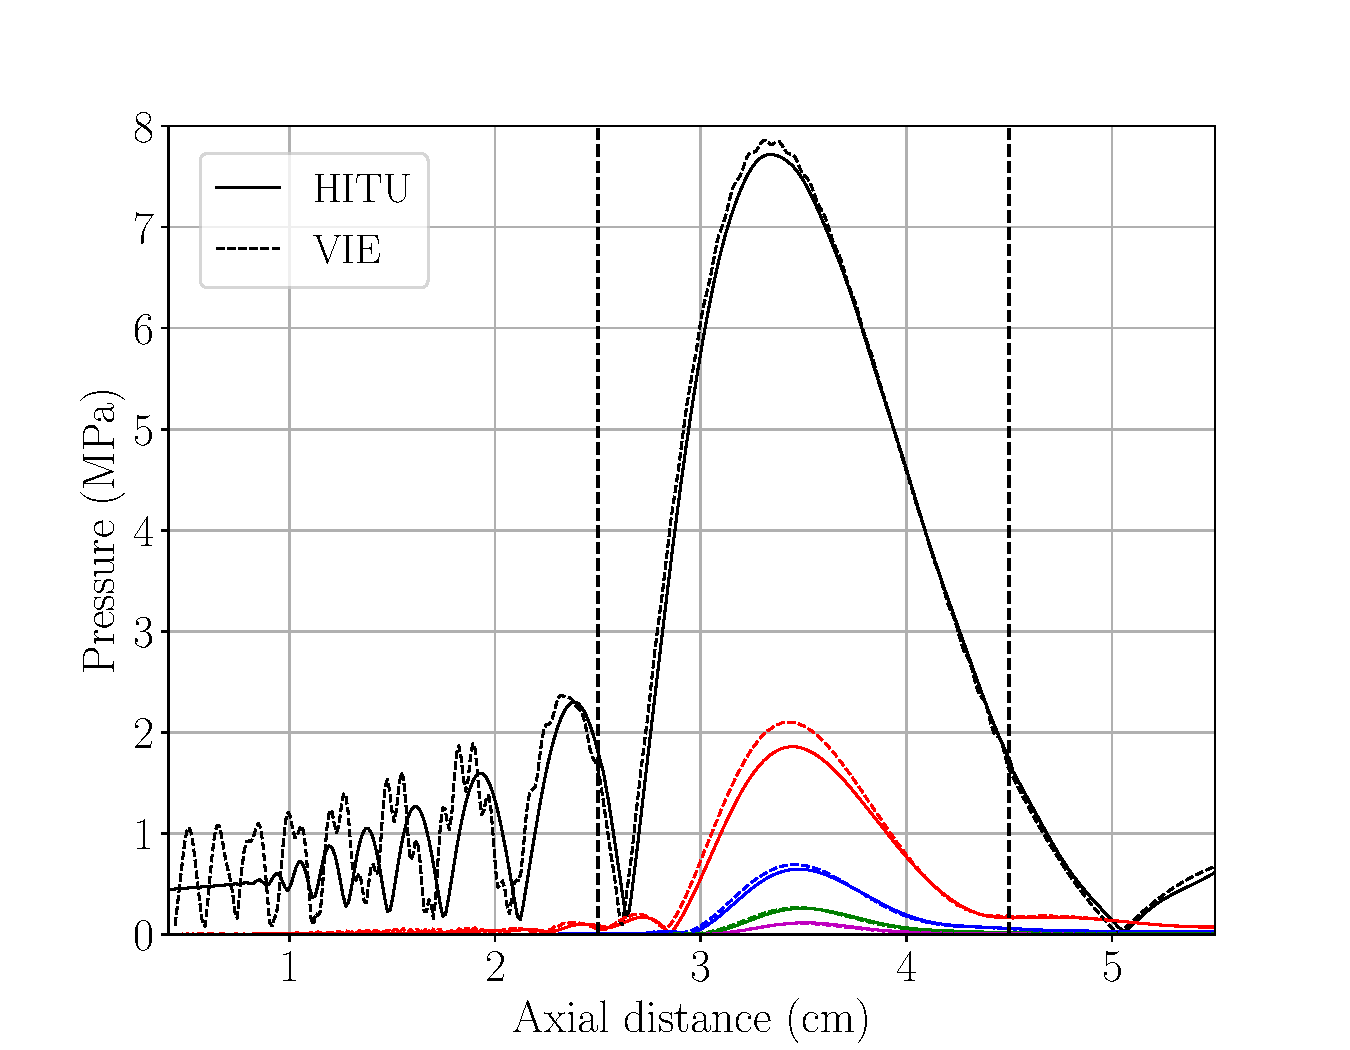
\includegraphics[width=\linewidth]{Figure12}
    \caption{The on-axis absolute pressure field for the first five harmonics generated 
    by the H131 transducer at 50W in water with a 2cm layer of kidney material centred 
    at 3.5cm. The vertical dashed lines demarcate the kidney layer.}
    \label{fig:HITU_comparison_slab}
\end{figure}  

We note that in the above we assumed that $\rho(\bx)\approx\rho_0$ throughout 
the inhomogeneous domain. This was done in order to derive convenient volume integral 
equations, which can be solved in an efficient manner. For strong density contrasts, 
the VIEs (\ref{eqn:harm1_inhomo})-(\ref{eqn:harm5_inhomo}) must be augmented with 
\textit{boundary integrals}, as discussed in \cite{costabel2015spectrum}. This 
complicated could be resolved by a coupling to an established boundary element code, such 
as \cite{van2015fast}, but this is left to future work.
}

%%%%%%%%%%%%%%%%%%%%%%%%%%%%%%%%%%%%%%%%%%%%%%%%%%%%%%%%%%%%%%%%%%%%%%%%%%%%%
\section{\label{sec:conclusion}Conclusion}
In this paper we have set out to reduce the computational burden of numerical 
schemes for \red{FUS} simulations through the construction of an efficient and simple 
meshing strategy. This strategy can be employed with those numerical schemes that 
\red{seek to approximate the Westervelt equation on a single non-uniform mesh}, and those that solve 
for each harmonic on separate meshes, such as the frequency-domain volume potential 
approach proposed here.

The strategy exploits the increasingly localised nature of the higher harmonics 
around the transducer's focal region so that the degrees of freedom in the mesh
can be more efficiently distributed. If we were considering a single non-uniform mesh approach 
\red{in which we approximate the full Westervelt equation}, this mesh would become 
increasingly more refined toward the focus, since this is where the higher 
harmonics are present. In the frequency-domain setting we considered, this leads to a nested 
series of meshes, as was discussed in detail in this article.

In the frequency domain, the Westervelt equation can be rewritten as a series 
of inhomogeneous Helmholtz equations. When the propagation medium is taken to be 
homogeneous, these Helmholtz equations can be solved exactly by volume potentials, 
which may be efficiently evaluated using the quadrature method proposed in 
Section~\ref{sec:volume}. This novel application of this approach allows us to 
explore efficiently the convergence of each harmonic as the respective computation 
domain was changed in size. Thus enabling us to determine the smallest domains 
we could use in order to achieve an error of less than 1\%.

We showed that the accurate approximation of the second harmonic requires a 
computation domain that extends from the focus all the way to the transducer, since 
the first harmonic is not sufficiently localised near the focus to allow a 
smaller domain to be employed. The third harmonic and above, however, can be 
approximated accurately on considerably reduced domains. We found that 
scaling the computation domain's width and height relative to the wavelength 
under consideration allowed for accurate approximations for the first five 
harmonics for the \red{FUS} configurations considered here. This leads to a reduction 
in the number of degrees of freedom of approximately $(n/2)^3$, where $n$ is 
the number of harmonics being computed.

\red{Finally, we demonstrated how this approach generalises, via the introduction of volume integral operators,
 to inhomogeneous media with low density variation.
The application to inhomogeneous media with large density contrast, such as between 
water and bone, requires the introduction of further boundary integral operators, 
with is left to future work.}

\red{To conclude, we briefly comment on the generalisation of the `rule of thumb'
to other transducer configurations and frequencies. In the present article, two 
different transducers were considered, both at 1.1MHz, and propagating within 
three different media: water, liver, kidney. All the examples considered produced 
peak amplitudes of lower than 15MPa, at which the weakly nonlinear assumption used 
in the derivation of the cascade of Helmholtz equations is accurate. We believe that 
for different focused transducer configurations and frequencies, our proposed rule 
of thumb is accurate, provided the field can still be categorised as weakly nonlinear.
For highly nonlinear fields, a further study would be required to test the `rule of 
thumb', and also a modification of our volume potential approach required to allow for 
the transfer of energy from higher to lower harmonics.}

% In addition to being of use to finite element methods, the volume potential 
% approach could be extended to inhomogeneous/scattering configurations by the 
% introduction of boundary and volume integral operators. Such an extension is 
% left to future work.

A Python implementation of this work is freely available at 
\begin{center}
    \verb!github.com/samuelpgroth/vines!.
\end{center}



% \begin{acknowledgments}
\section*{Acknowledgments}
This work was supported by a grant entitled 
``Optimising patient specific treatment plans for ultrasound ablative therapies in the abdomen (OptimUS)''
from the EPSRC (EP/P013309/1 to Cambridge, EP/P012434/1 to UCL).
%The grant title is ``Optimising patient specific treatment plans for ultrasound ablative therapies in the abdomen (OptimUS)''.
% \end{acknowledgments}


\bibliographystyle{acm} 
\bibliography{Cambridge_bib}

\end{document}